\documentclass[letterpaper,10pt]{article}
\usepackage[margin=2cm]{geometry}

\usepackage{graphicx}
\usepackage{amsmath}
\usepackage{amsfonts}
\usepackage{amssymb}
\usepackage{multicol}
\usepackage{listings}
\usepackage{color}

\definecolor{mygreen}{rgb}{0,0.6,0}
\definecolor{mygray}{rgb}{0.5,0.5,0.5}
\definecolor{mymauve}{rgb}{0.58,0,0.82}

\lstset{ %
  backgroundcolor=\color{white},   % choose the background color; you must add \usepackage{color} or \usepackage{xcolor}
  basicstyle=\footnotesize,        % the size of the fonts that are used for the code
  breakatwhitespace=false,         % sets if automatic breaks should only happen at whitespace
  breaklines=true,                 % sets automatic line breaking
  captionpos=b,                    % sets the caption-position to bottom
  commentstyle=\color{mygreen},    % comment style
  deletekeywords={...},            % if you want to delete keywords from the given language
  escapeinside={\%*}{*)},          % if you want to add LaTeX within your code
  extendedchars=true,              % lets you use non-ASCII characters; for 8-bits encodings only, does not work with UTF-8
  frame=single,	                   % adds a frame around the code
  keepspaces=true,                 % keeps spaces in text, useful for keeping indentation of code (possibly needs columns=flexible)
  keywordstyle=\color{blue},       % keyword style
  language=Matlab,                 % the language of the code
  otherkeywords={},           % if you want to add more keywords to the set
  numbers=left,                    % where to put the line-numbers; possible values are (none, left, right)
  numbersep=5pt,                   % how far the line-numbers are from the code
  numberstyle=\tiny\color{mygray}, % the style that is used for the line-numbers
  rulecolor=\color{black},         % if not set, the frame-color may be changed on line-breaks within not-black text (e.g. comments (green here))
  showspaces=false,                % show spaces everywhere adding particular underscores; it overrides 'showstringspaces'
  showstringspaces=false,          % underline spaces within strings only
  showtabs=false,                  % show tabs within strings adding particular underscores
  stepnumber=1,                    % the step between two line-numbers. If it's 1, each line will be numbered
  stringstyle=\color{mymauve},     % string literal style
  tabsize=4,	                   % sets default tabsize to 2 spaces
  title=\lstname                   % show the filename of files included with \lstinputlisting; also try caption instead of title
}

\DeclareMathOperator*{\argmin}{arg\,min}
\DeclareMathOperator*{\argmax}{arg\,max}

\title{\textbf{Pattern Recognition Theory 18794 Homework 2}}
\author{Mengwen He (Alex)}

\begin{document}

\maketitle

\section*{Problem 1}

PCA vs LDA. Given the following dataset for a 2-class problem with 2-D features:

\begin{equation}
\nonumber
c_1=\left\{\left[\begin{array}{c}
2 \\ 1
\end{array}\right],\left[\begin{array}{c}
2 \\ 2
\end{array}\right],\left[\begin{array}{c}
2 \\ 3
\end{array}\right]\right\},~
c_2=\left\{\left[\begin{array}{c}
4 \\ 3
\end{array}\right],\left[\begin{array}{c}
5 \\ 3
\end{array}\right],\left[\begin{array}{c}
6 \\ 4
\end{array}\right]\right\}
\end{equation}

\begin{enumerate}
\item Using global PCA, find the best direction onto which the data will be projected on.\\
\lstinputlisting[language=Matlab]{./matlab/P_1_1.m}
\begin{enumerate}
	\item Express the equation of the line along this direction passing	through the samples mean in the following form: $\vec{w}^T\vec{x} + w_0 = 0$, where
	$$\vec{x}=\left[\begin{array}{c}
	x_1 \\ x_2
	\end{array}\right]\text{~and~}\vec{w}=\left[\begin{array}{c}
	w_1 \\ w_2
	\end{array}\right]$$
	and $w_0$ is a scalar known as the bias. Plot the $\vec{w}^T\vec{x} + w0 = 0$ line
	along with all the sample points as well the line along $\vec{w}$ which recall starts from the mean.
	$$\vec{w}=\left[\begin{array}{c}
	 0.4541 \\
	 -0.8910 \\
	\end{array}\right],~w_0=0.7866$$
	
	\item Project and reconstruct all the sample points. Plot the reconstructed points.
	\begin{center}
	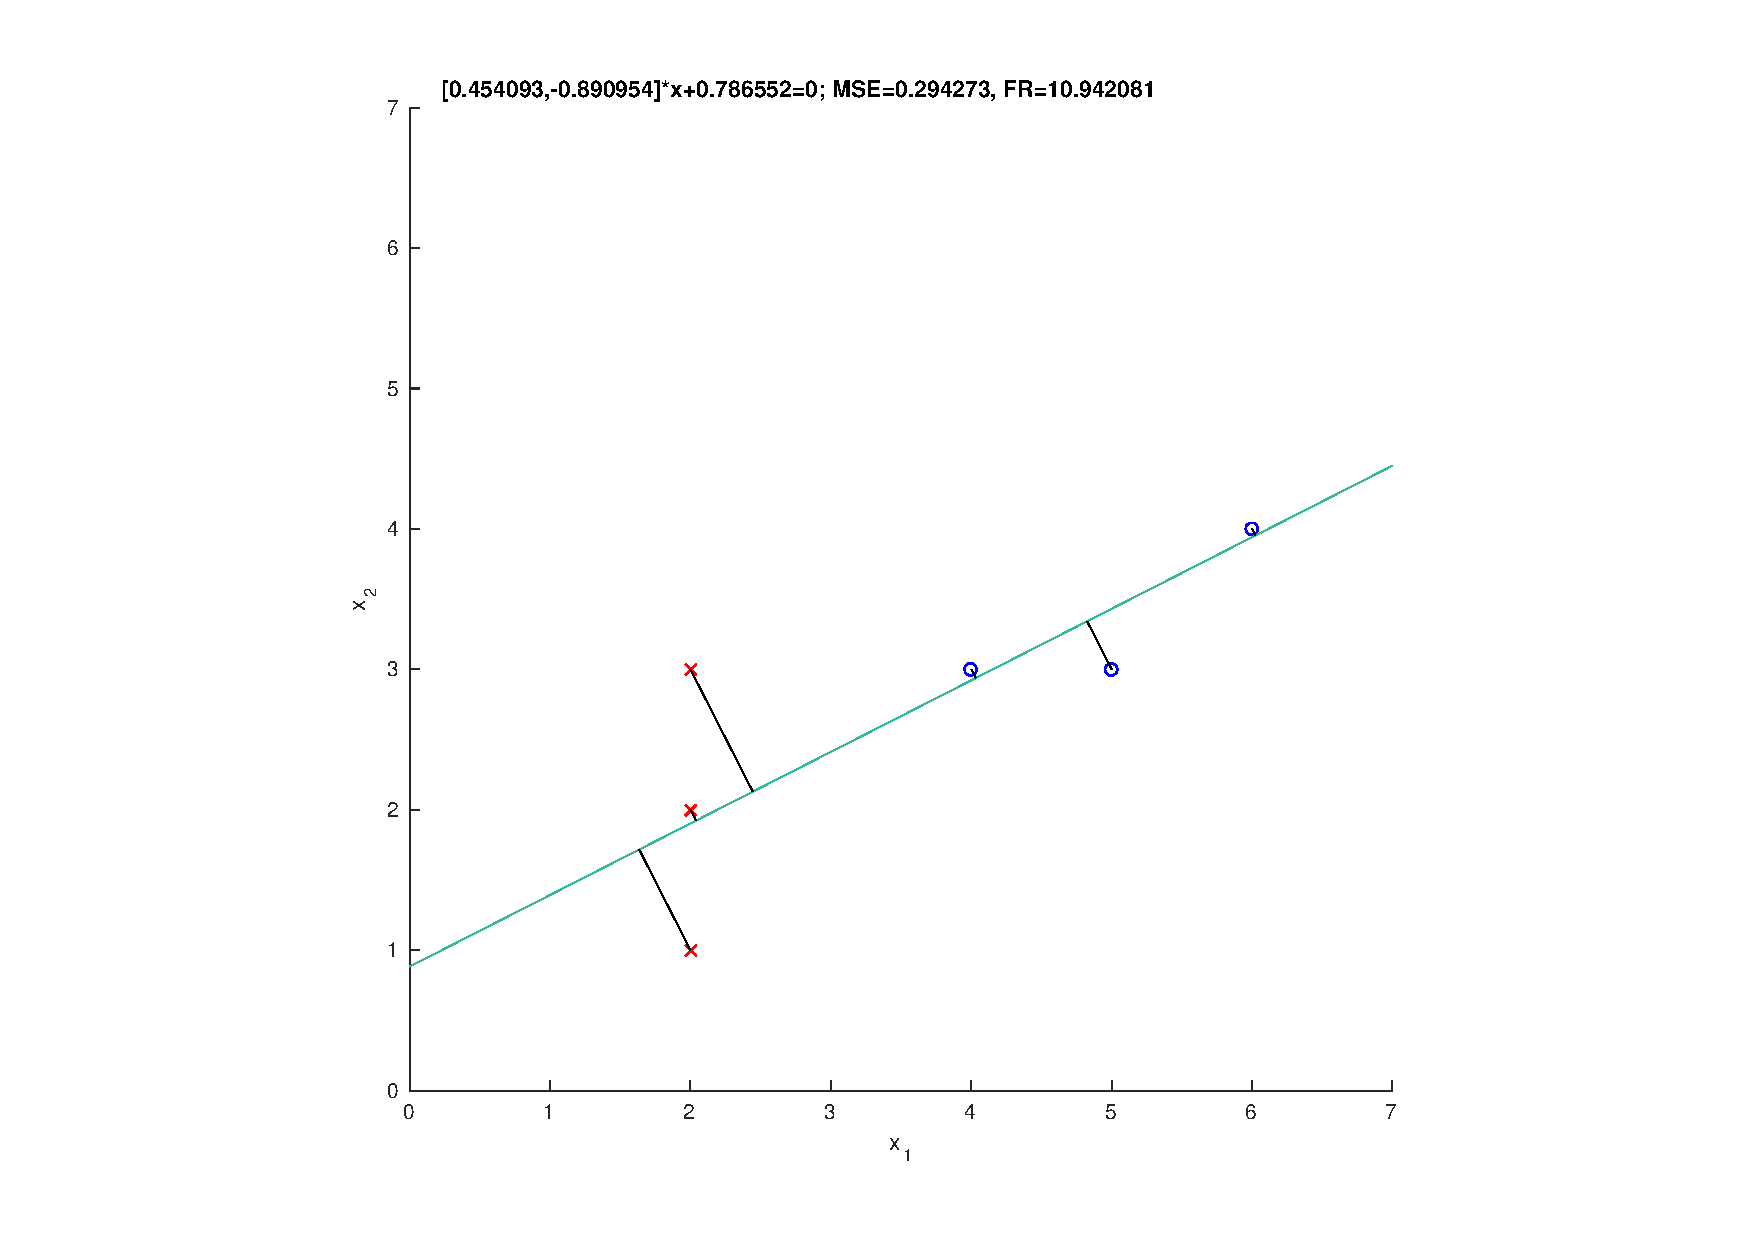
\includegraphics[width=0.65\textwidth]{./matlab/PCA.eps}
	\end{center}
	
	
	\item Find the total mean square error MSE for all sample points (between the original points and the reconstructed points).
	$$MSE=0.2943$$
	
	\item Find the Fisher Ratio for this projection defined by
	$$FR=\frac{(m_1-m_2)^2}{\sigma_1^2+\sigma_2^2}$$
	where $m_i$ is the mean of the projected samples of class $i$, and $\sigma_i^2$ is the equivalent variance. You can compute the $FR$ on the projected 1-D points (rather than the reconstructed points which are 2-D vectors).
	$$FR=10.9421$$
	
\end{enumerate}

\item Using Fisher Linear Discriminant Analysis (LDA), determine the best one-dimensional space onto which the above data should be projected.\\
\lstinputlisting[language=Matlab]{./matlab/P_1_2.m}
\begin{enumerate}
	\item Express the equation of the line along this direction passing
	through the samples mean in the following form: $\vec{w}^T\vec{x}+w0 = 0$. Plot
	the $\vec{w}^T\vec{x} + w0 = 0$ line along with all the sample points.
	$$\vec{w}=\left[\begin{array}{c}
		 -0.0499 \\
		    -0.9988 \\
		\end{array}\right],~w_0=2.8381$$
	
	\item Project and reconstruct all the sample points. Plot the reconstructed points. Make sure they lie on a line.\\
	\begin{center}
		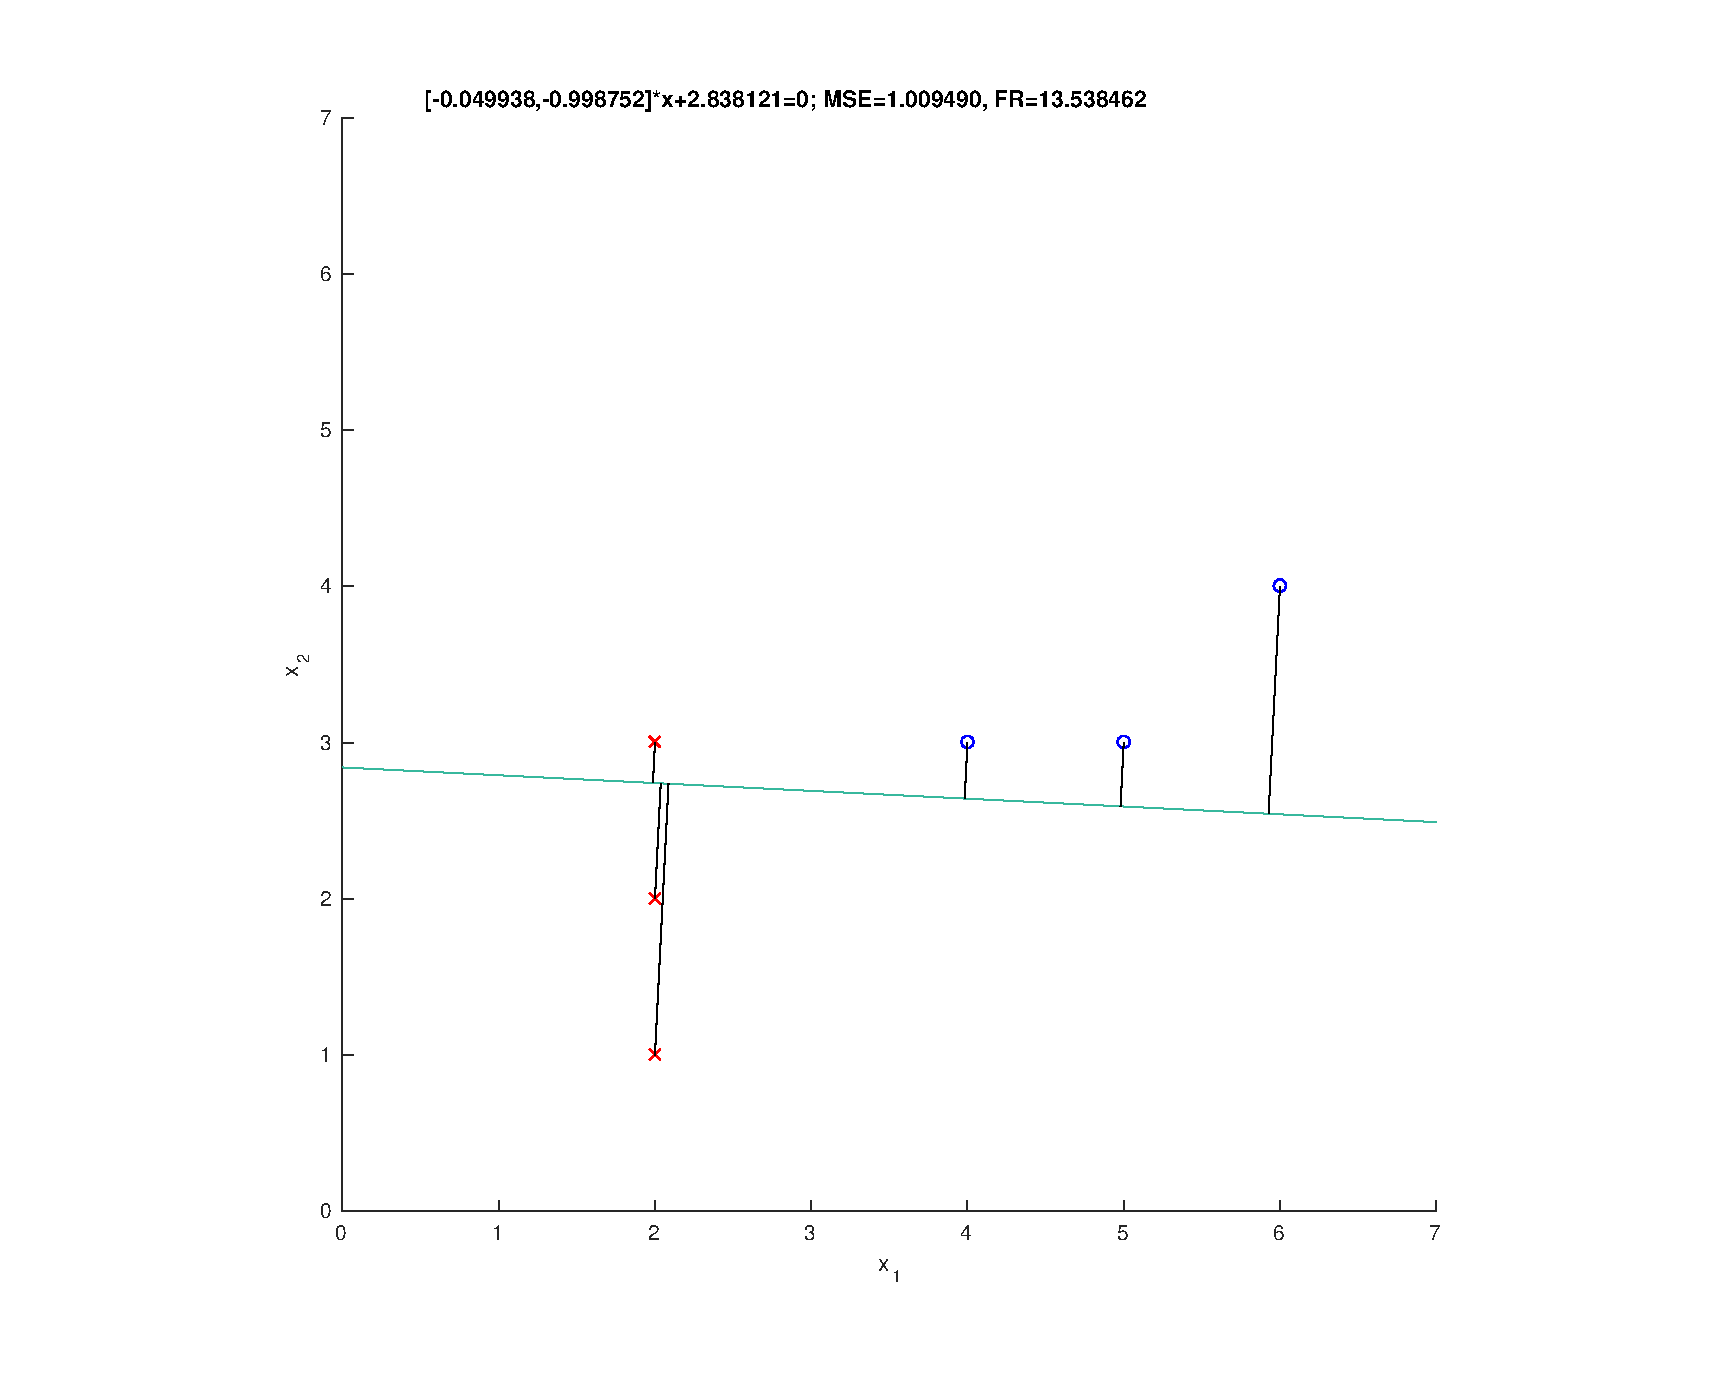
\includegraphics[width=0.65\textwidth]{./matlab/LDA.eps}
	\end{center}
	
	\item Find the total MSE for all sample points (between the original points and the reconstructed points). Compare that to the total MSE found in the first question.
	$$MSE=1.0095$$
	
	\item Find the Fisher Ratio for this projection. You can compute the FR on the projected points (rather than the reconstructed points which are 2-D vectors). Compare that to the $FR$ found in part 1. Interpret your result.
	$$FR=13.5385$$
	
\end{enumerate}
\end{enumerate}

\section*{Problem 2}

Another goal of PCA is to obtain the linear subspace which minimizes the projection error caused by dimension reduction. The two goals, maximum variance and minimum error, have the same formulation as PCA.

\begin{enumerate}
\item Assume all data samples $\{\vec{x}_1,\dots,\vec{x}_n\}$ are centered. Formulate the optimization problem to solve for a vector $\vec{w}$ spanning the linear subspace which minimizes the sum of the squared reconstruction errors:
$$\sum_{i=1}^{n}{d_i^2}$$
where $d_i$, the reconstruction error of $\vec{x}_i$, is defined as the distance between $\vec{x}_i$ and its projection onto the linear subspace. Assume that $\vec{w}$ has a unit norm since we are interested only in the direction of the vector $\vec{w}$. The answer must be written in terms of $\vec{w}$ and $\vec{x}_i$ without $d_i$.\\
\textbf{Answer:}\\
$\because$
\begin{equation}
\nonumber
\begin{array}{rcl}
d_i^2(\vec{w}) & = & ||\vec{x}_i-\vec{w}\vec{x}_i^T\vec{w}||_2^2 \\
 & = & (\vec{x}_i-\vec{w}\vec{x}_i^T\vec{w})^T(\vec{x}_i-\vec{w}\vec{x}_i^T\vec{w}) \\
 & = & \vec{x}_i^T\vec{x}_i-2\vec{x}_i^T\vec{w}\vec{x}_i^T\vec{w}+\vec{w}^T\vec{x}_i\vec{x}_i^T\vec{w}\\
 & = & \vec{x}_i^T\vec{x}_i-2\vec{w}^T(\vec{x}_i\vec{x}_i^T)\vec{w}+\vec{w}^T(\vec{x}_i\vec{x}_i^T)\vec{w}\\
 & = & \vec{x}_i^T\vec{x}_i-\vec{w}^T(\vec{x}_i\vec{x}_i^T)\vec{w}\\
 \sum_{i=1}^{n}{d_i^2(\vec{w})} & = & \sum_{i=1}^{n}{\vec{x}_i^T\vec{x}_i}-\vec{w}^T\sum_{i=1}^{n}{(\vec{x}_i\vec{x}_i^T)}\vec{w} \\
 \text{where}~~||\vec{w}|| & = & 1 \\
 & = & \vec{w}^T\vec{w}=1 
\end{array}
\end{equation}
$\therefore$ use Lagrange Multipliers to get the optimized $\vec{w}$:
\begin{equation}
\nonumber
\begin{array}{rcl}
L(\vec{w},\lambda) & = & \sum_{i=1}^{n}{d_i^2(\vec{w})} - \lambda(1-\vec{w}^T\vec{w}) \\
 & = & \sum_{i=1}^{n}{\vec{x}_i^T\vec{x}_i}-\vec{w}^T\sum_{i=1}^{n}{(\vec{x}_i\vec{x}_i^T)}\vec{w} - \lambda(1-\vec{w}^T\vec{w}) \\
 \frac{\partial L}{\partial \lambda} & = & \vec{w}^T\vec{w}-1 = 0 \\
 \frac{\partial L}{\partial \vec{w}} & = & -2(\sum_{i=1}^{n}{\vec{x}_i\vec{x}_i^T})\vec{w}+2\lambda\vec{w} = 0\\
 & \Rightarrow & \left(\sum_{i=1}^{n}{\vec{x}_i\vec{x}_i^T}\right)\vec{w}=\lambda\vec{w} \\
\end{array}
\end{equation}
$\therefore$ $\lambda$s are the eigenvalues, and $\vec{w}$s are the corresponding eigenvectors of $\sum_{i=1}^{n}{\vec{x}_i\vec{x}_i^T}$.\\
$\because$
$$\left(\sum_{i=1}^{n}{\vec{x}_i\vec{x}_i^T}\right)\vec{w}=\lambda\vec{w}\Rightarrow\vec{w}^T\left(\sum_{i=1}^{n}{\vec{x}_i\vec{x}_i^T}\right)\vec{w}=\lambda$$
and
$$\sum_{i=1}^{n}{\vec{x}_i^T\vec{x}_i}\text{ is constant}$$
$\therefore$ to minimize $\sum_{i=1}^{n}{d_i^2(\vec{w})}$, we need to choose the $\vec{w}^*$ to maximize $\vec{w}^T\left(\sum_{i=1}^{n}{\vec{x}_i\vec{x}_i^T}\right)\vec{w}=\lambda=\lambda_{max}$.

\item From your answer in (a), show that the optimization in part (a) is equivalent to the PCA optimization using the following equivalence:
$$\Sigma = \sum_{i}^{n}{\vec{x}_i\vec{x}_i^T}$$
\textbf{Answer:}\\
$\because$ PCA is to choose the $\vec{w}^*$ to maximize the variant after projection $\vec{w}^T\Sigma\vec{w}=\lambda=\lambda_{max}$.\\
$\therefore$ they are equivalent.
\end{enumerate}



\section*{Problem 3}

You are to implement PCA from scratch and not use the MATLAB built in
functions. You are allowed to use SVD and/or eigenvalue decomposition. Please
submit a print out of your code aw well.

\begin{enumerate}
	\item Plot the mean image of digit 1 and plot the first 5 global PCA vectors
	corresponding to the dataset corresponding to two cases: using Gram
	Matrix Trick and without Gram Matrix trick. Do not forget to remove
	the mean before you run PCA. Measure the time taken for the PCA vector
	computation in each case.\\
	\lstinputlisting[language=Matlab]{./matlab/P_3_1.m}
	\begin{center}
	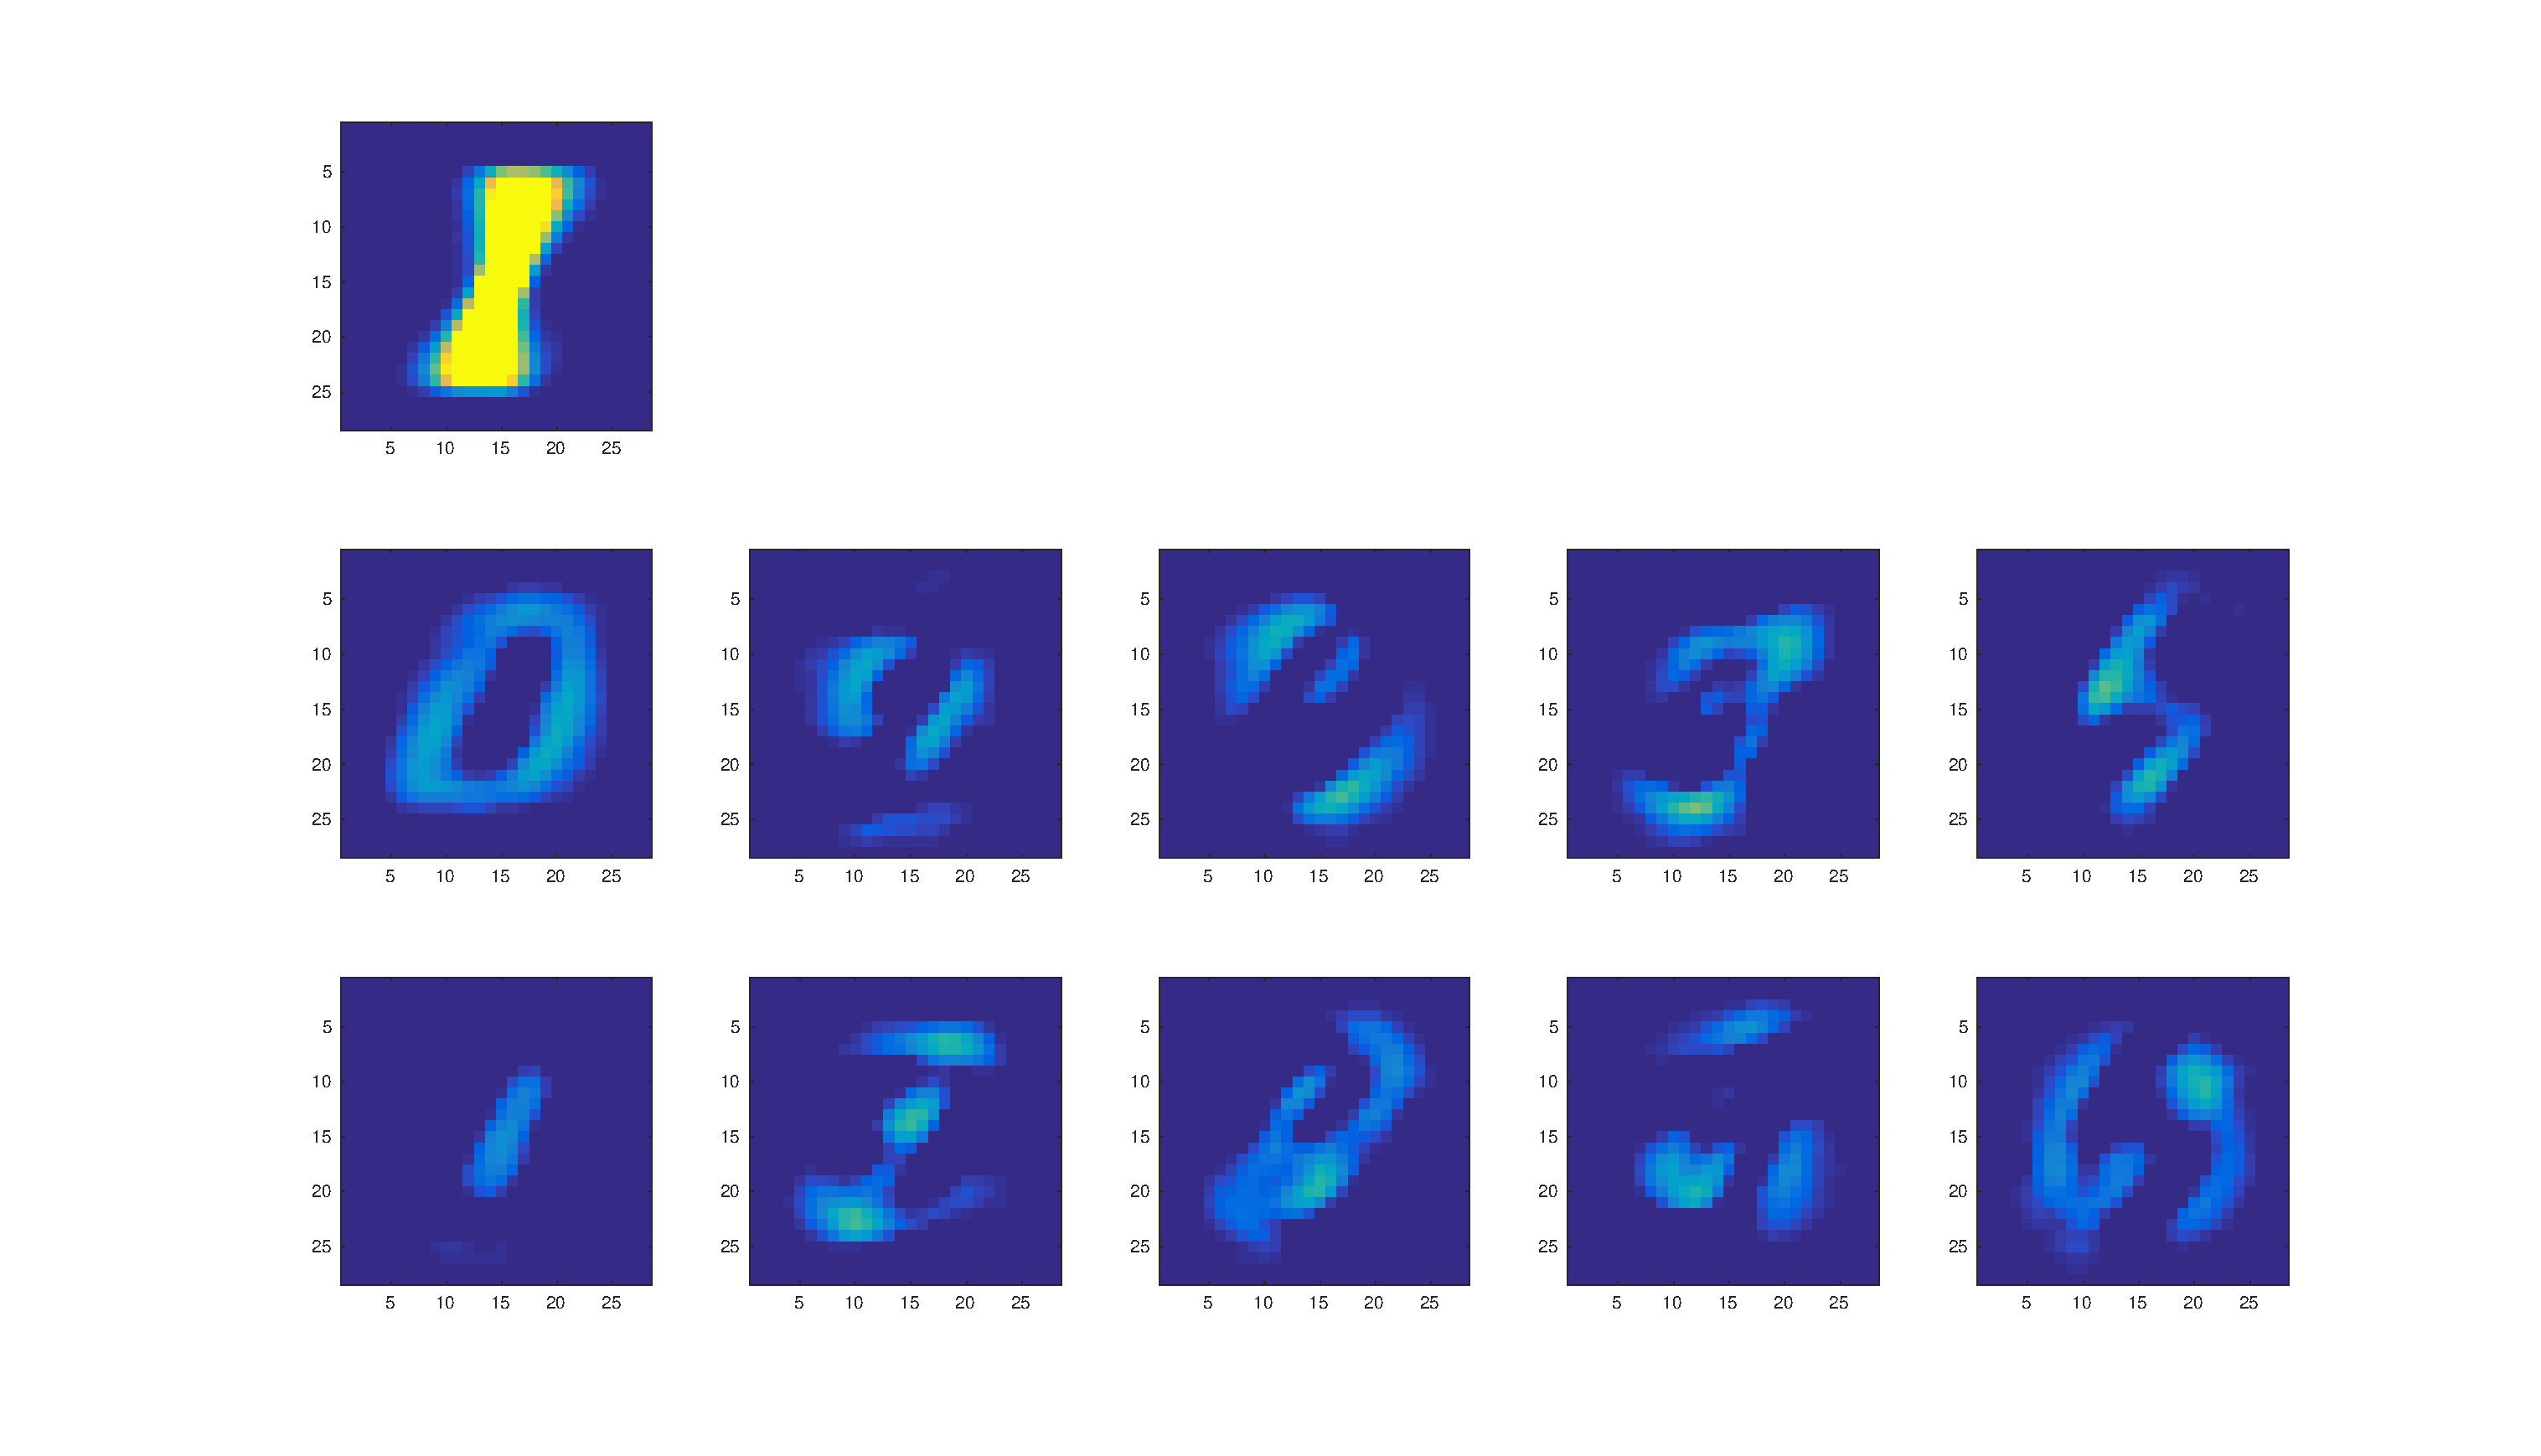
\includegraphics[width=0.9\textwidth]{./matlab/digit_1.eps}\\
	The first row is the digit 1's mean image; the second row is the first 5 eigenvector images without Gram trick; the third row is the first 5 eigenvector images with Gram trick.
	\end{center}
	
	\item Comment on the time taken in each case. Does it make sense to use the
	Gram trick for this particular dataset?\\
	\textbf{Answer:}
	\begin{itemize}
		\item When samplenum=1000 (total number is 1000*10=10000): w/o Gram costs 0.100550s, and w/ Gram costs 4.579334s.
		\item When samplenum=100 (total number is 100*10=1000): w/o Gram costs 0.037760s, and w/ Gram costs 0.038084s.
		\item When samplenum=10 (total number is 10*10=100): w/o Gram costs 0.013963s, and w/ Gram costs 0.042149s.
		\item When samplenum=1 (total number is 10*10=100): w/o Gram costs 0.008933s, and w/ Gram costs 0.003651s.
	\end{itemize}
	Therefore, if $N<<d$, Gram trick is helpful for the PCA algorithm speed.
	
	\item  Pick any random image from the dataset which can be any image from any
	class and project onto the eigen space (the global PCA eigen space that
	you obtained in part 1 of this problem) and reconstruct it using the first n
	eigen vectors (not just the nth vector but all of them up until n) (for the
	two cases, Gram trick and without it) where $n = \{1, 2, 5, 10, 20\}$. Do not
	forget to remove the mean before projecting the image, and also to add it
	back once it has been reconstructed using only the first n eigen vectors.
	
	For each of the 5 reconstructions, compute the mean square error (MSE)
	of the reconstructed image. Note that the MSE between two vectors $\vec{a}$
	and $\vec{b}$ is given by
	$$MSE(\vec{a},\vec{b})=||\vec{a}-\vec{b}||_2^2$$
	Display all reconstructed images and the original in one figure, with the
	corresponding MSE value as the title of each sub-figure\\
	\lstinputlisting[language=Matlab]{./matlab/P_3_3.m}
	\newpage
	\begin{center}
	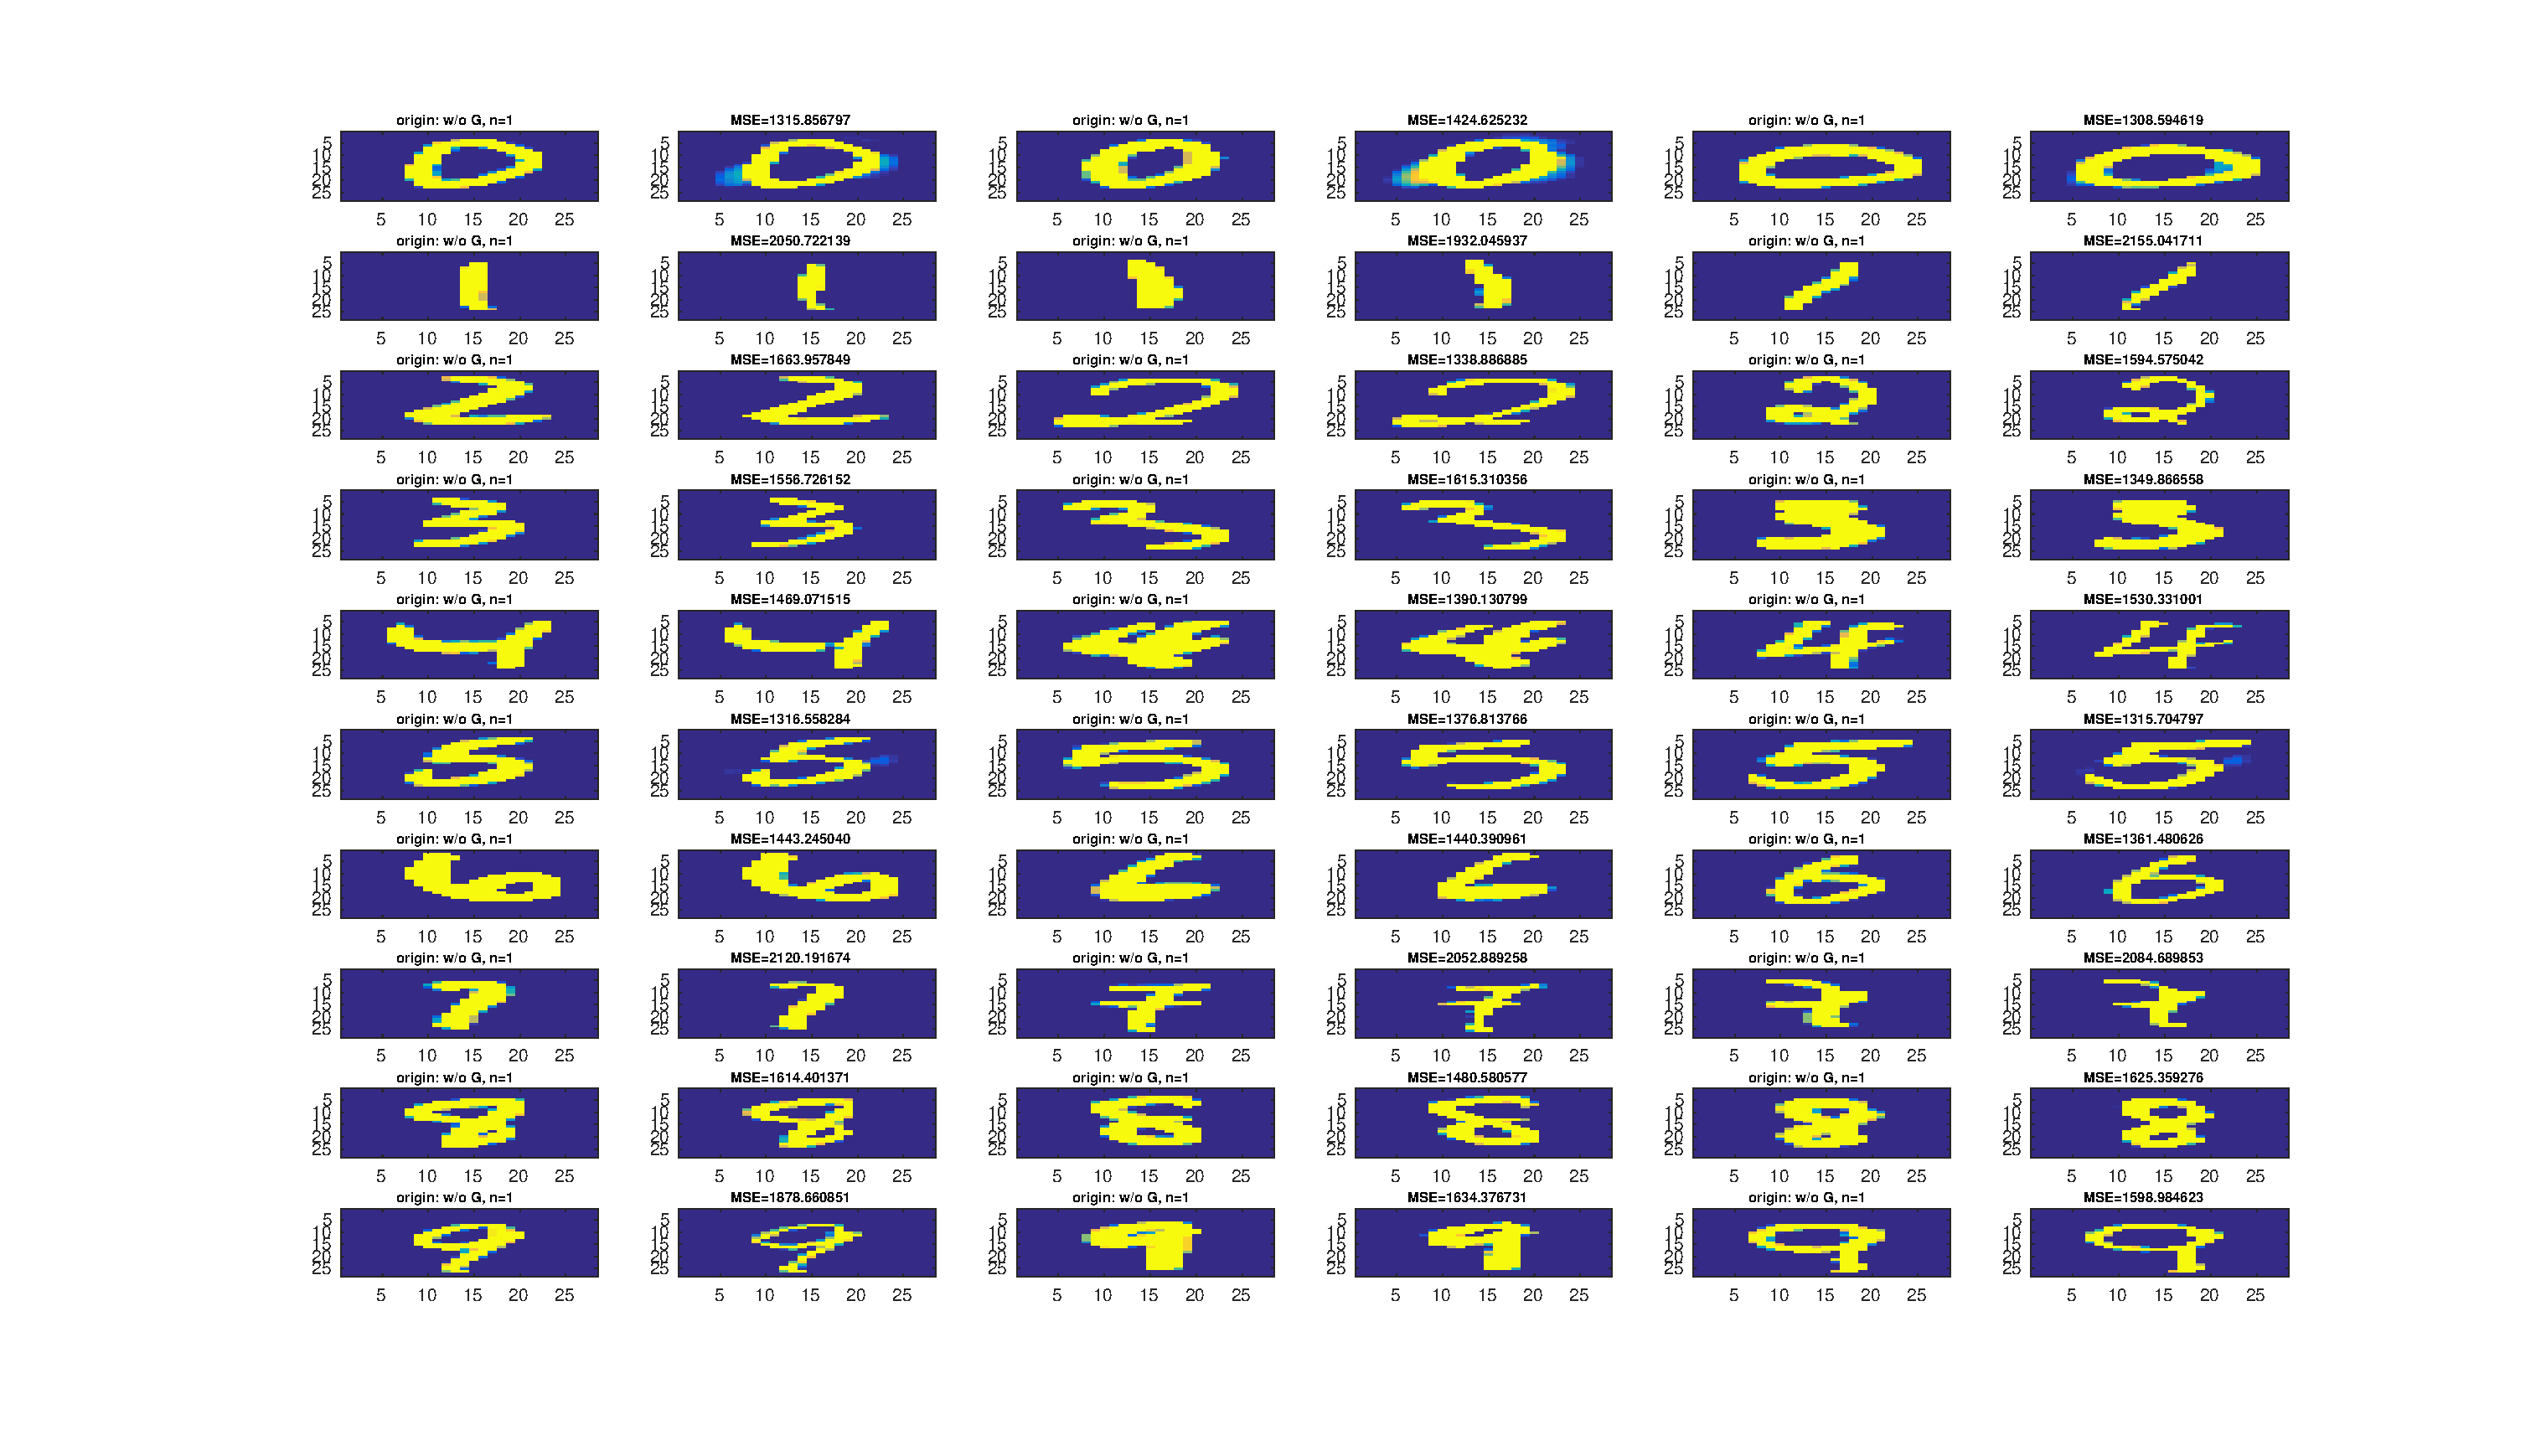
\includegraphics[width=0.95\textwidth]{./matlab/WoG_N01.eps}
	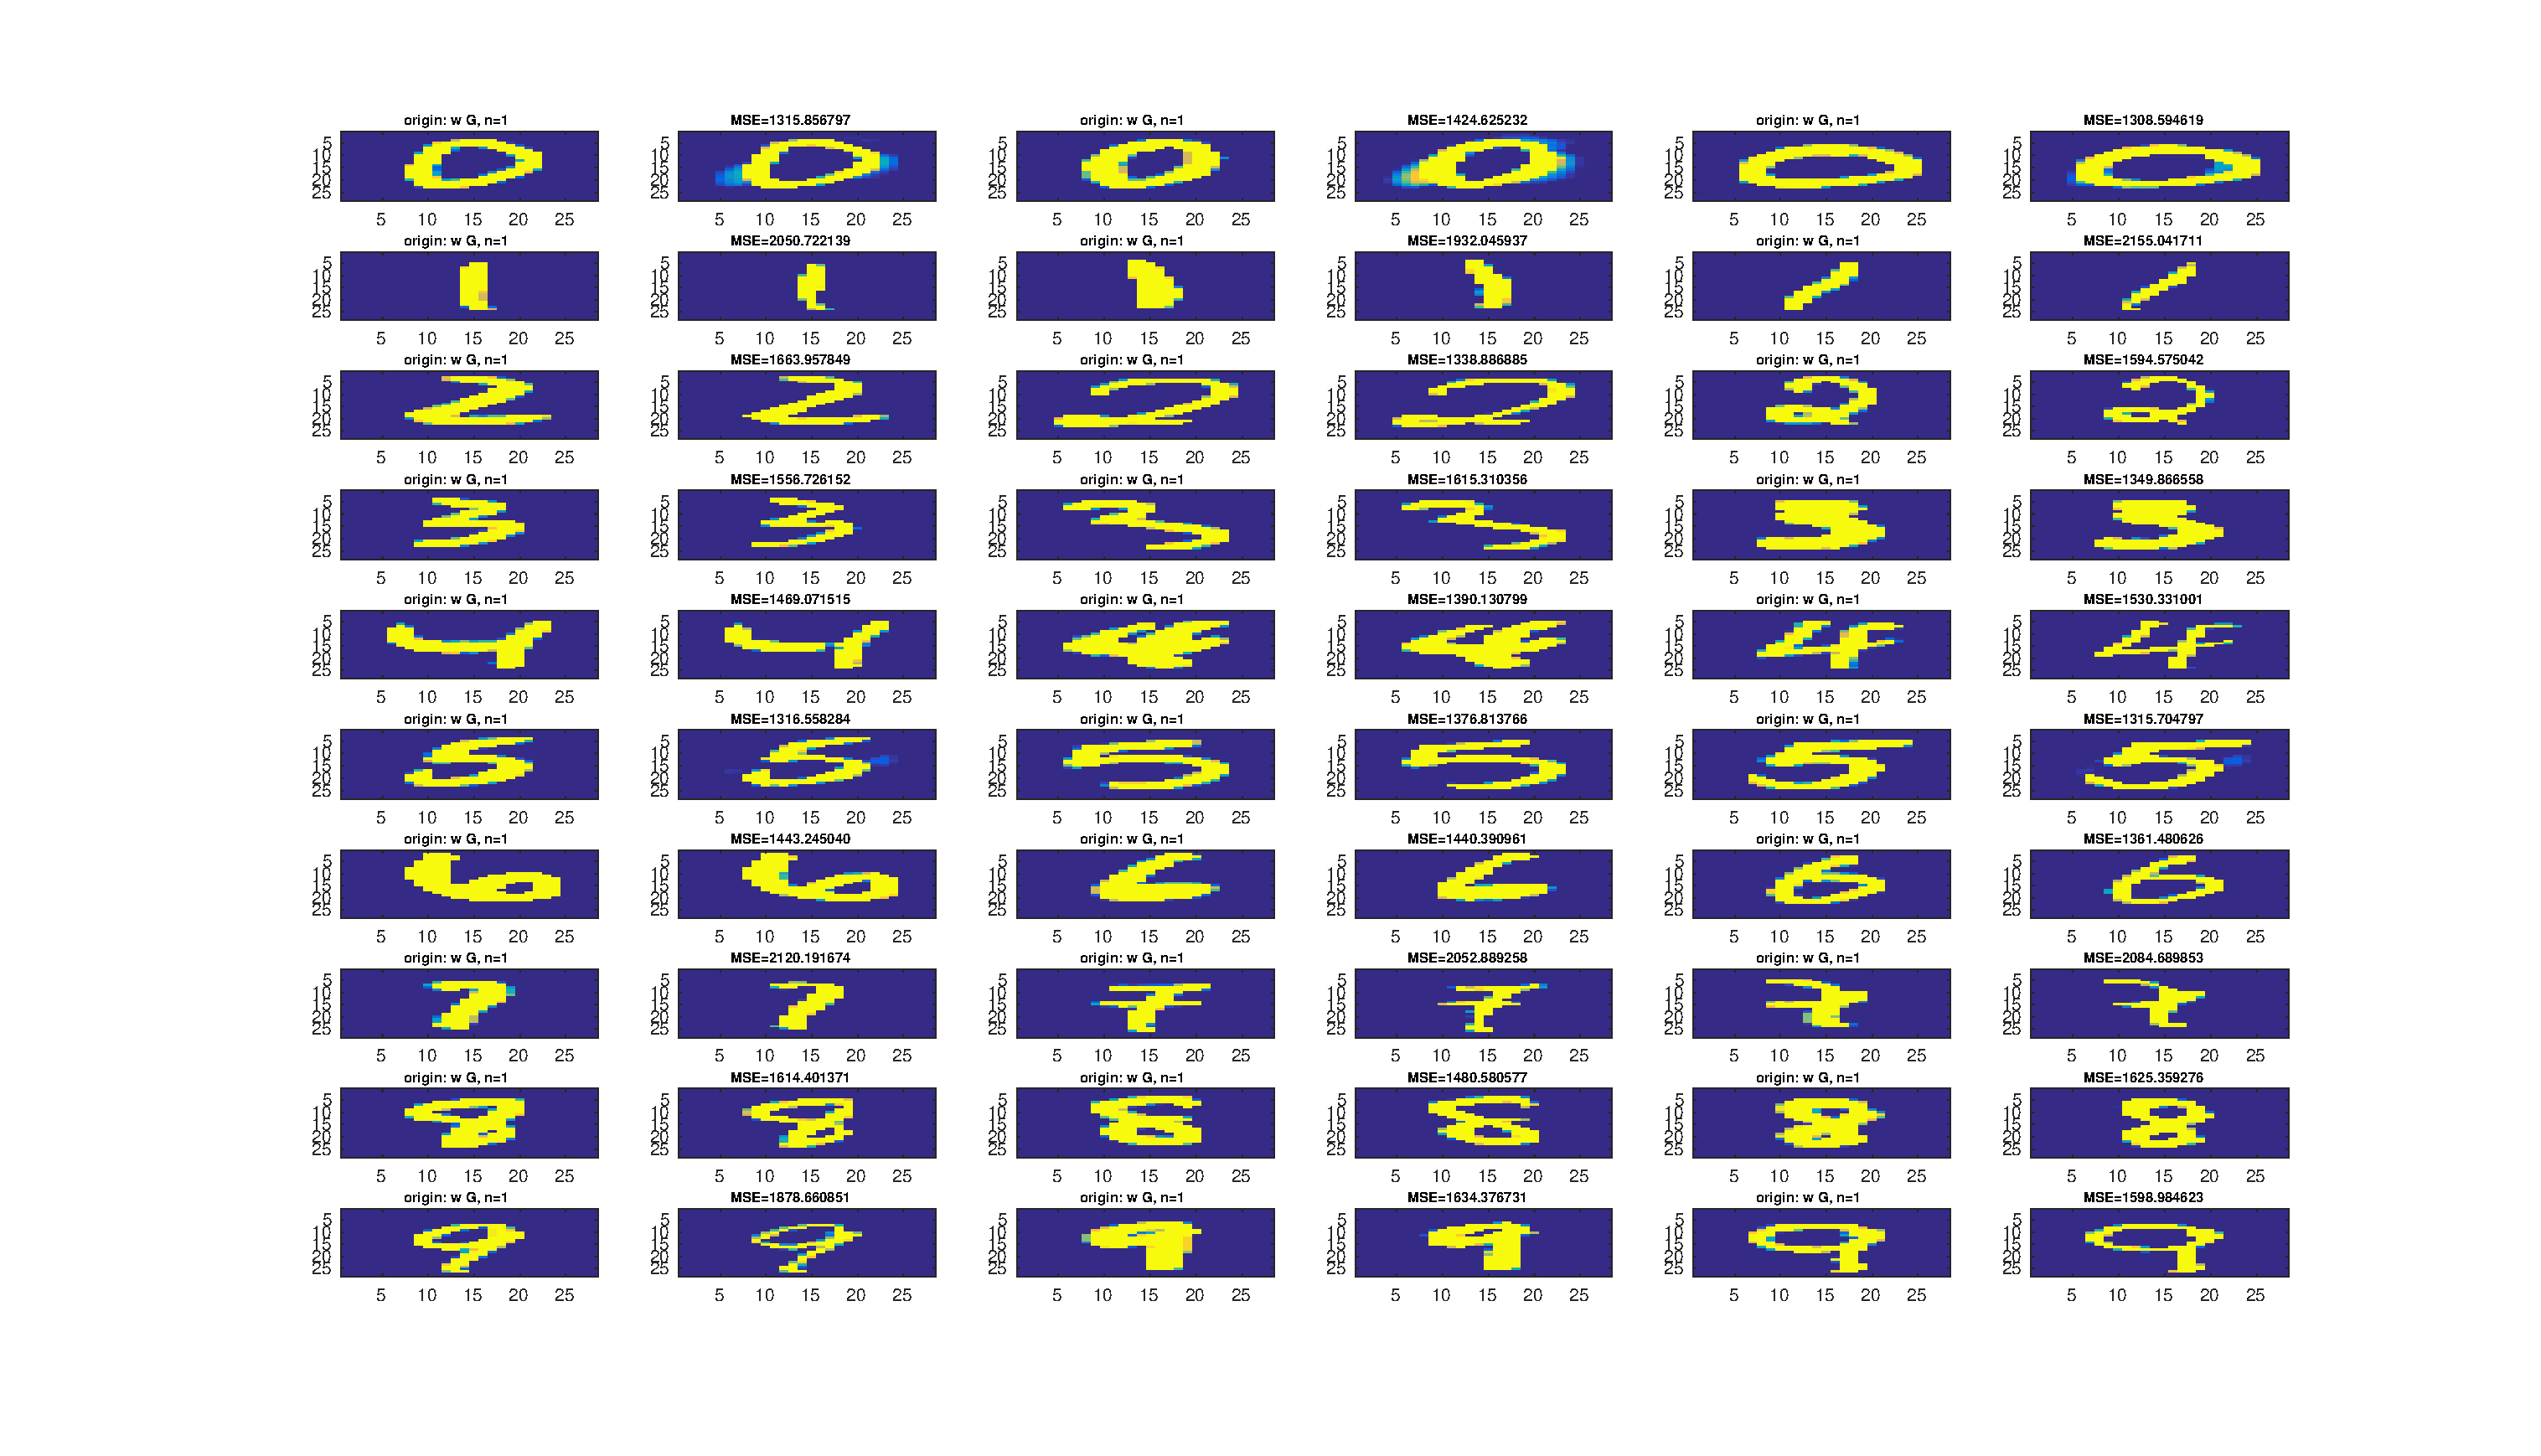
\includegraphics[width=0.95\textwidth]{./matlab/WG_N01.eps}
	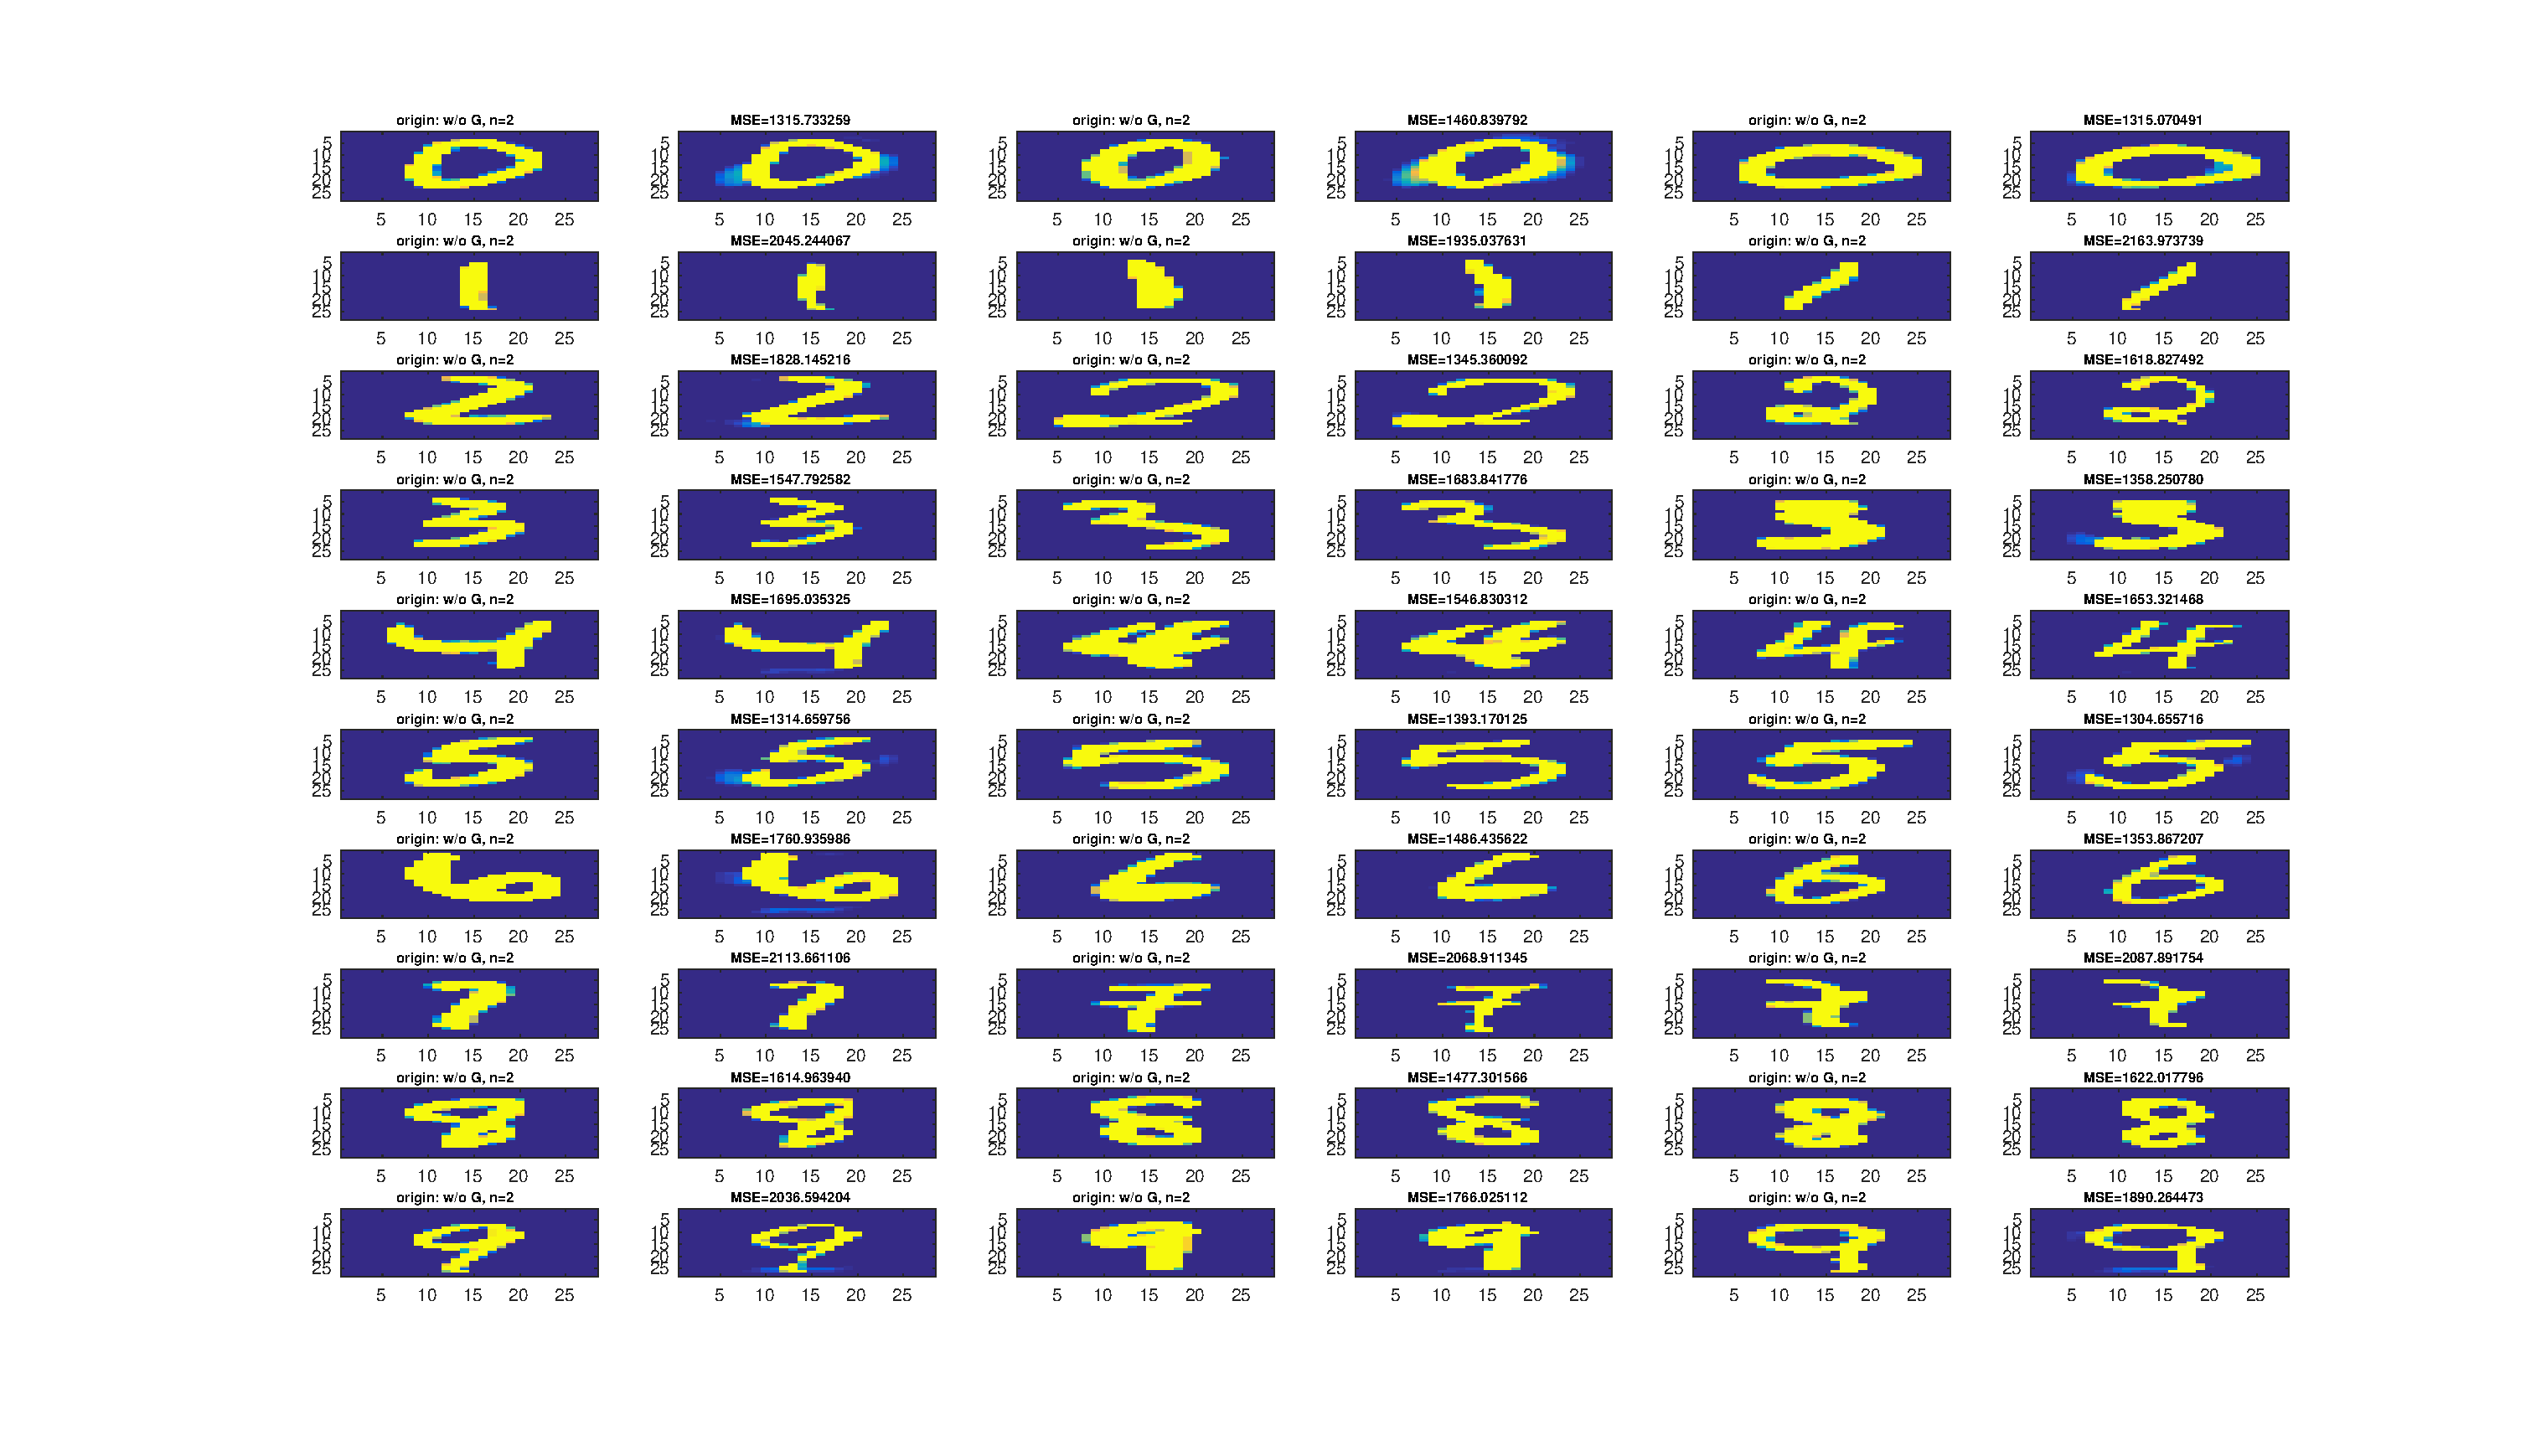
\includegraphics[width=0.95\textwidth]{./matlab/WoG_N02.eps}
	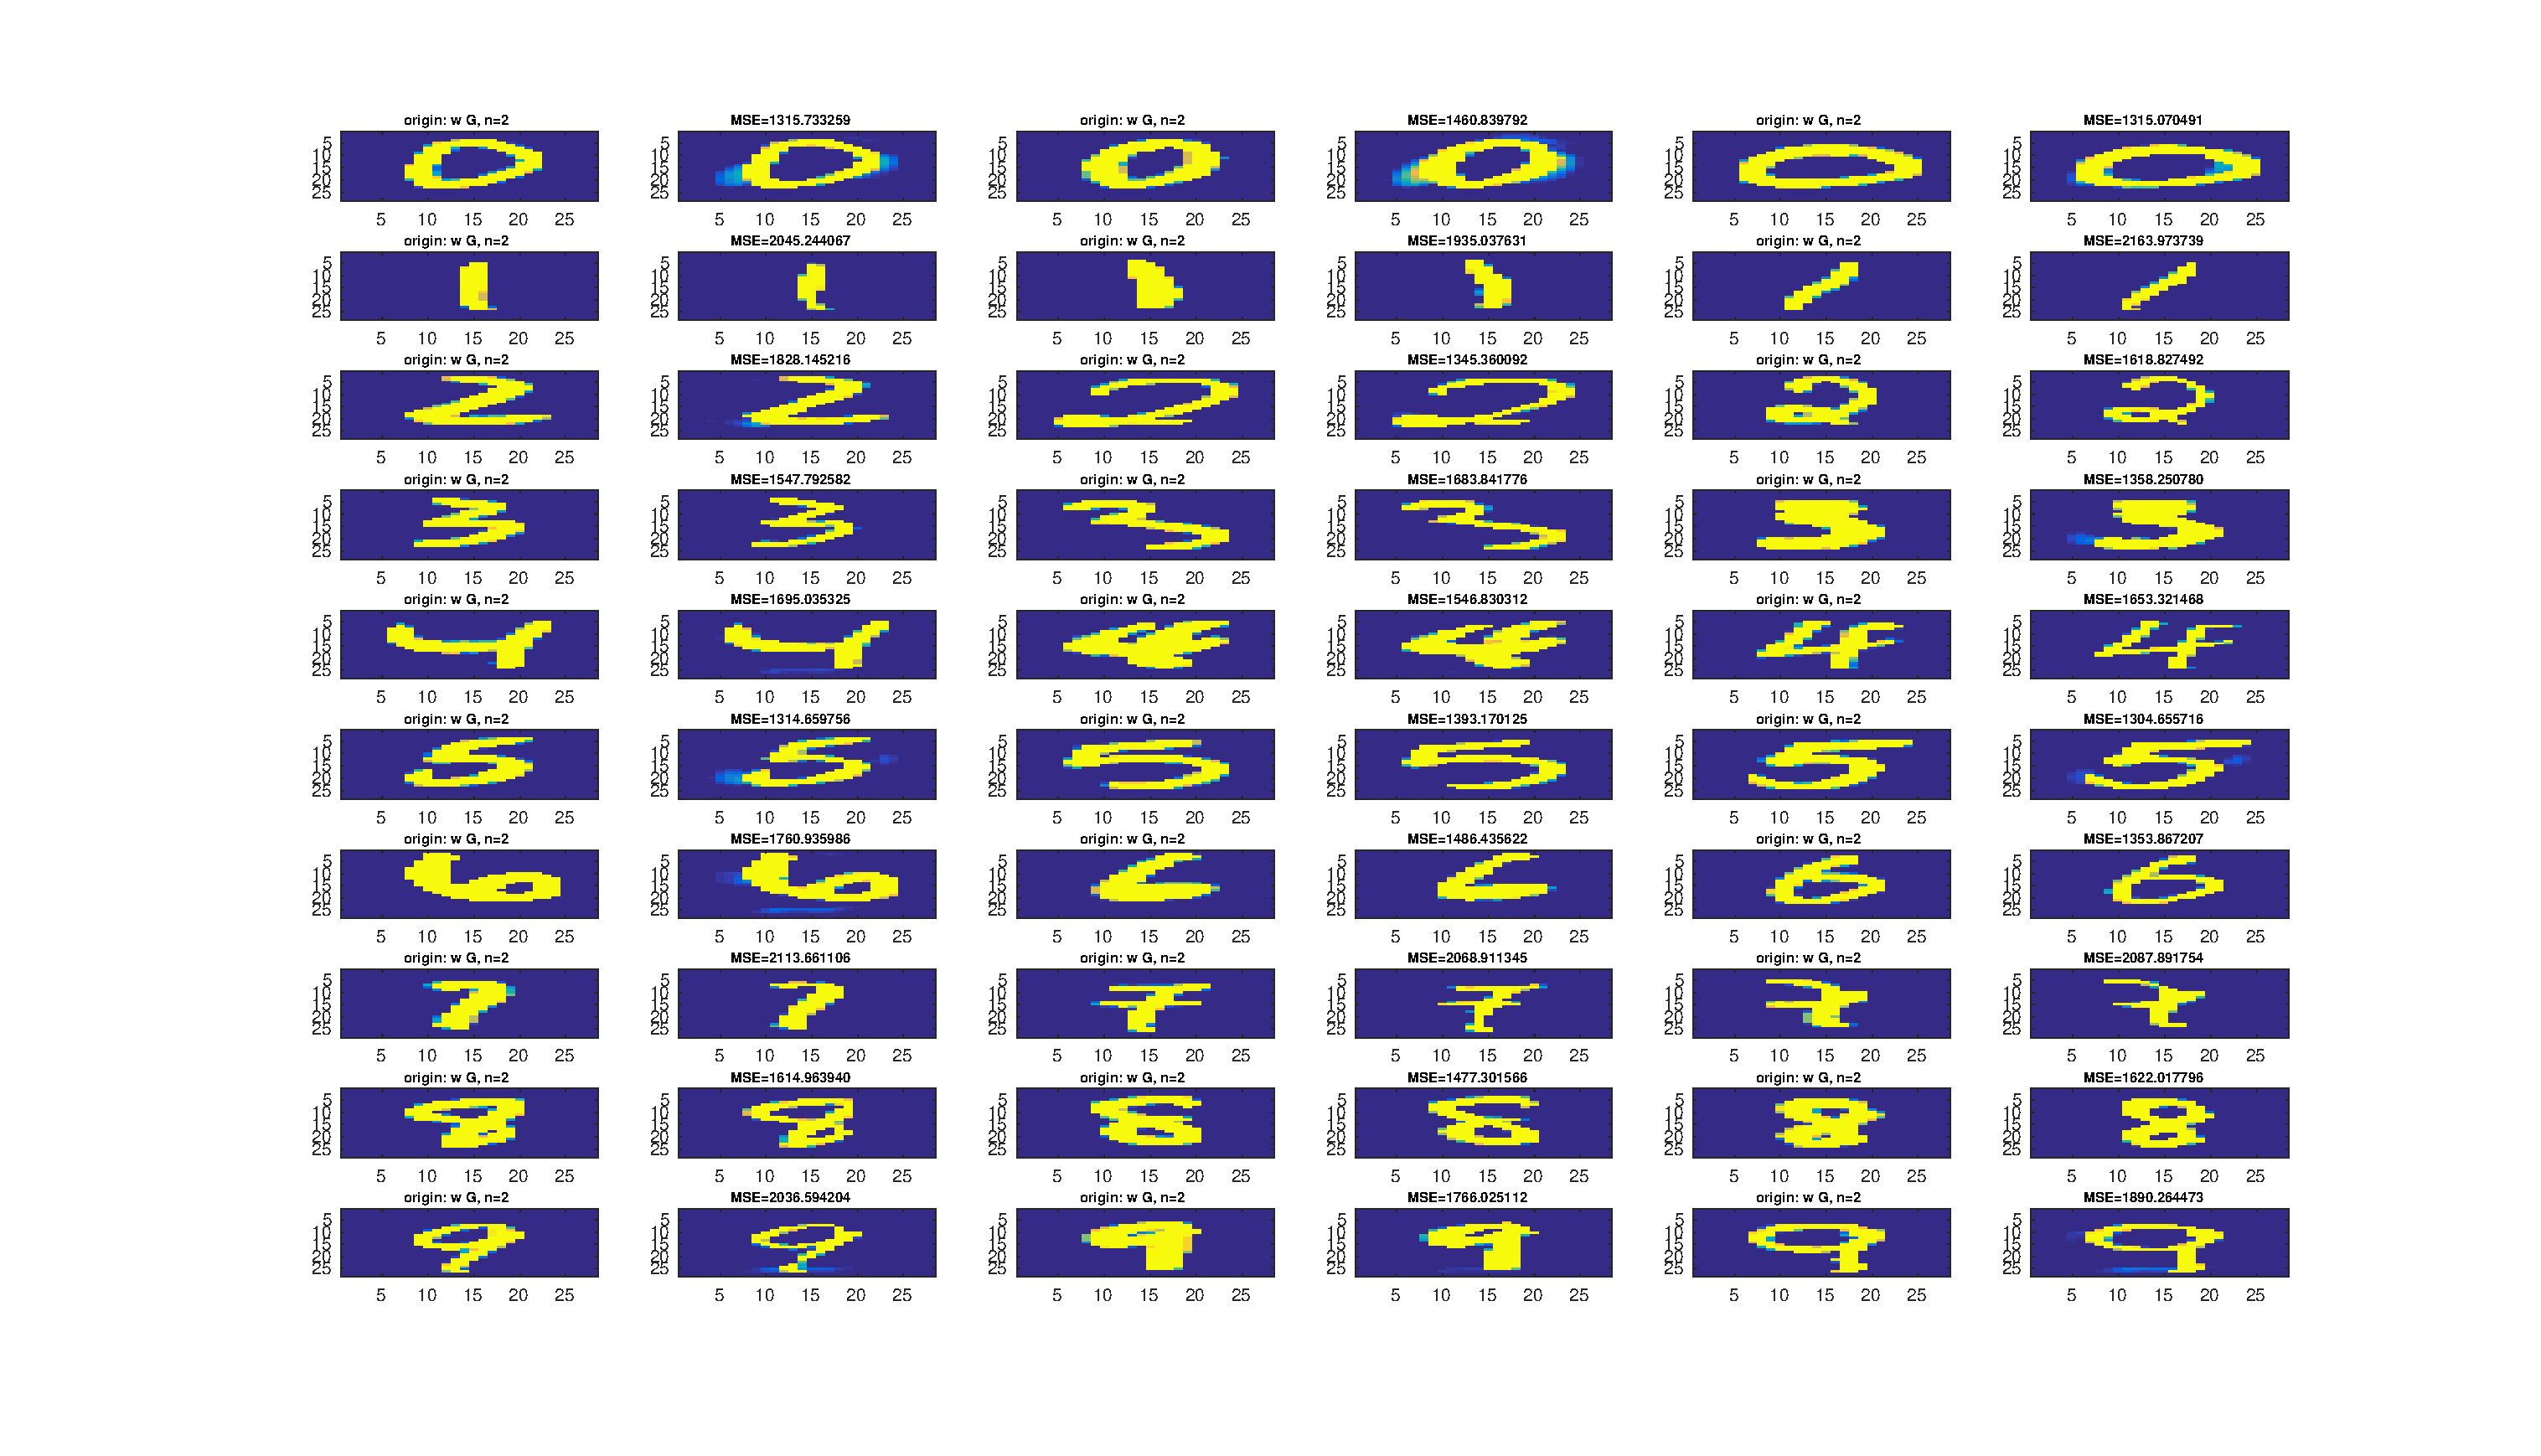
\includegraphics[width=0.95\textwidth]{./matlab/WG_N02.eps}
	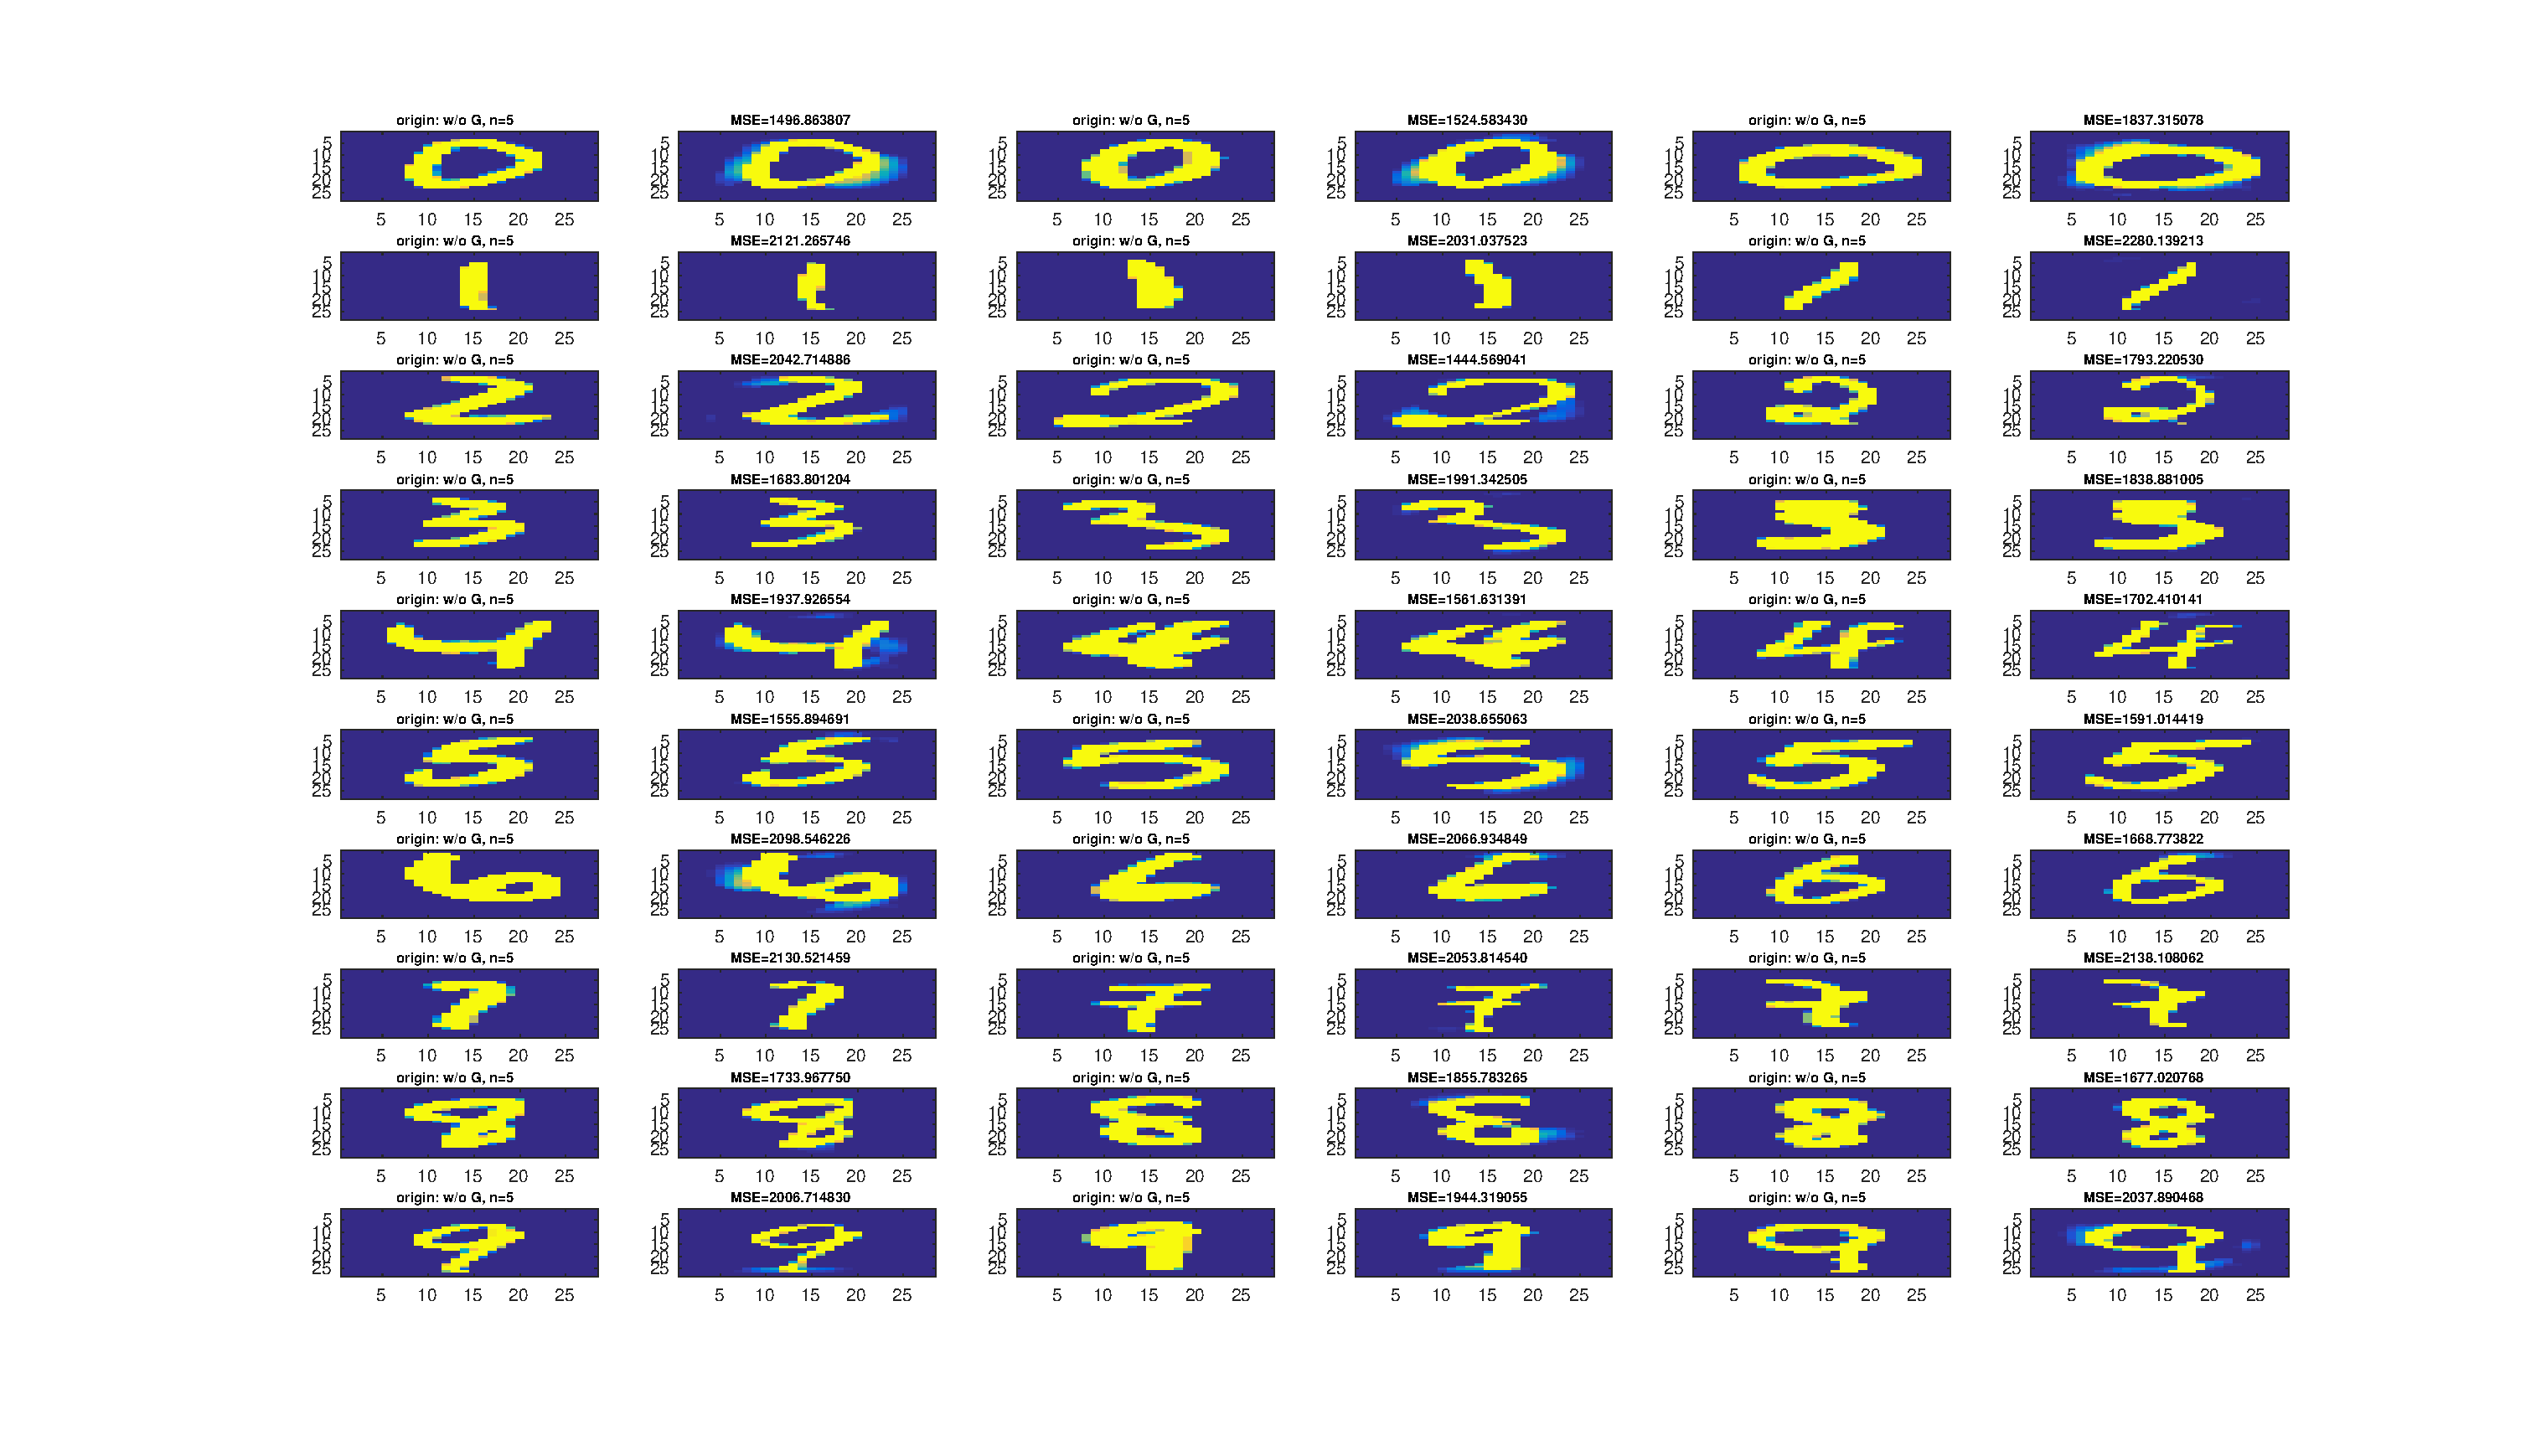
\includegraphics[width=0.95\textwidth]{./matlab/WoG_N05.eps}
	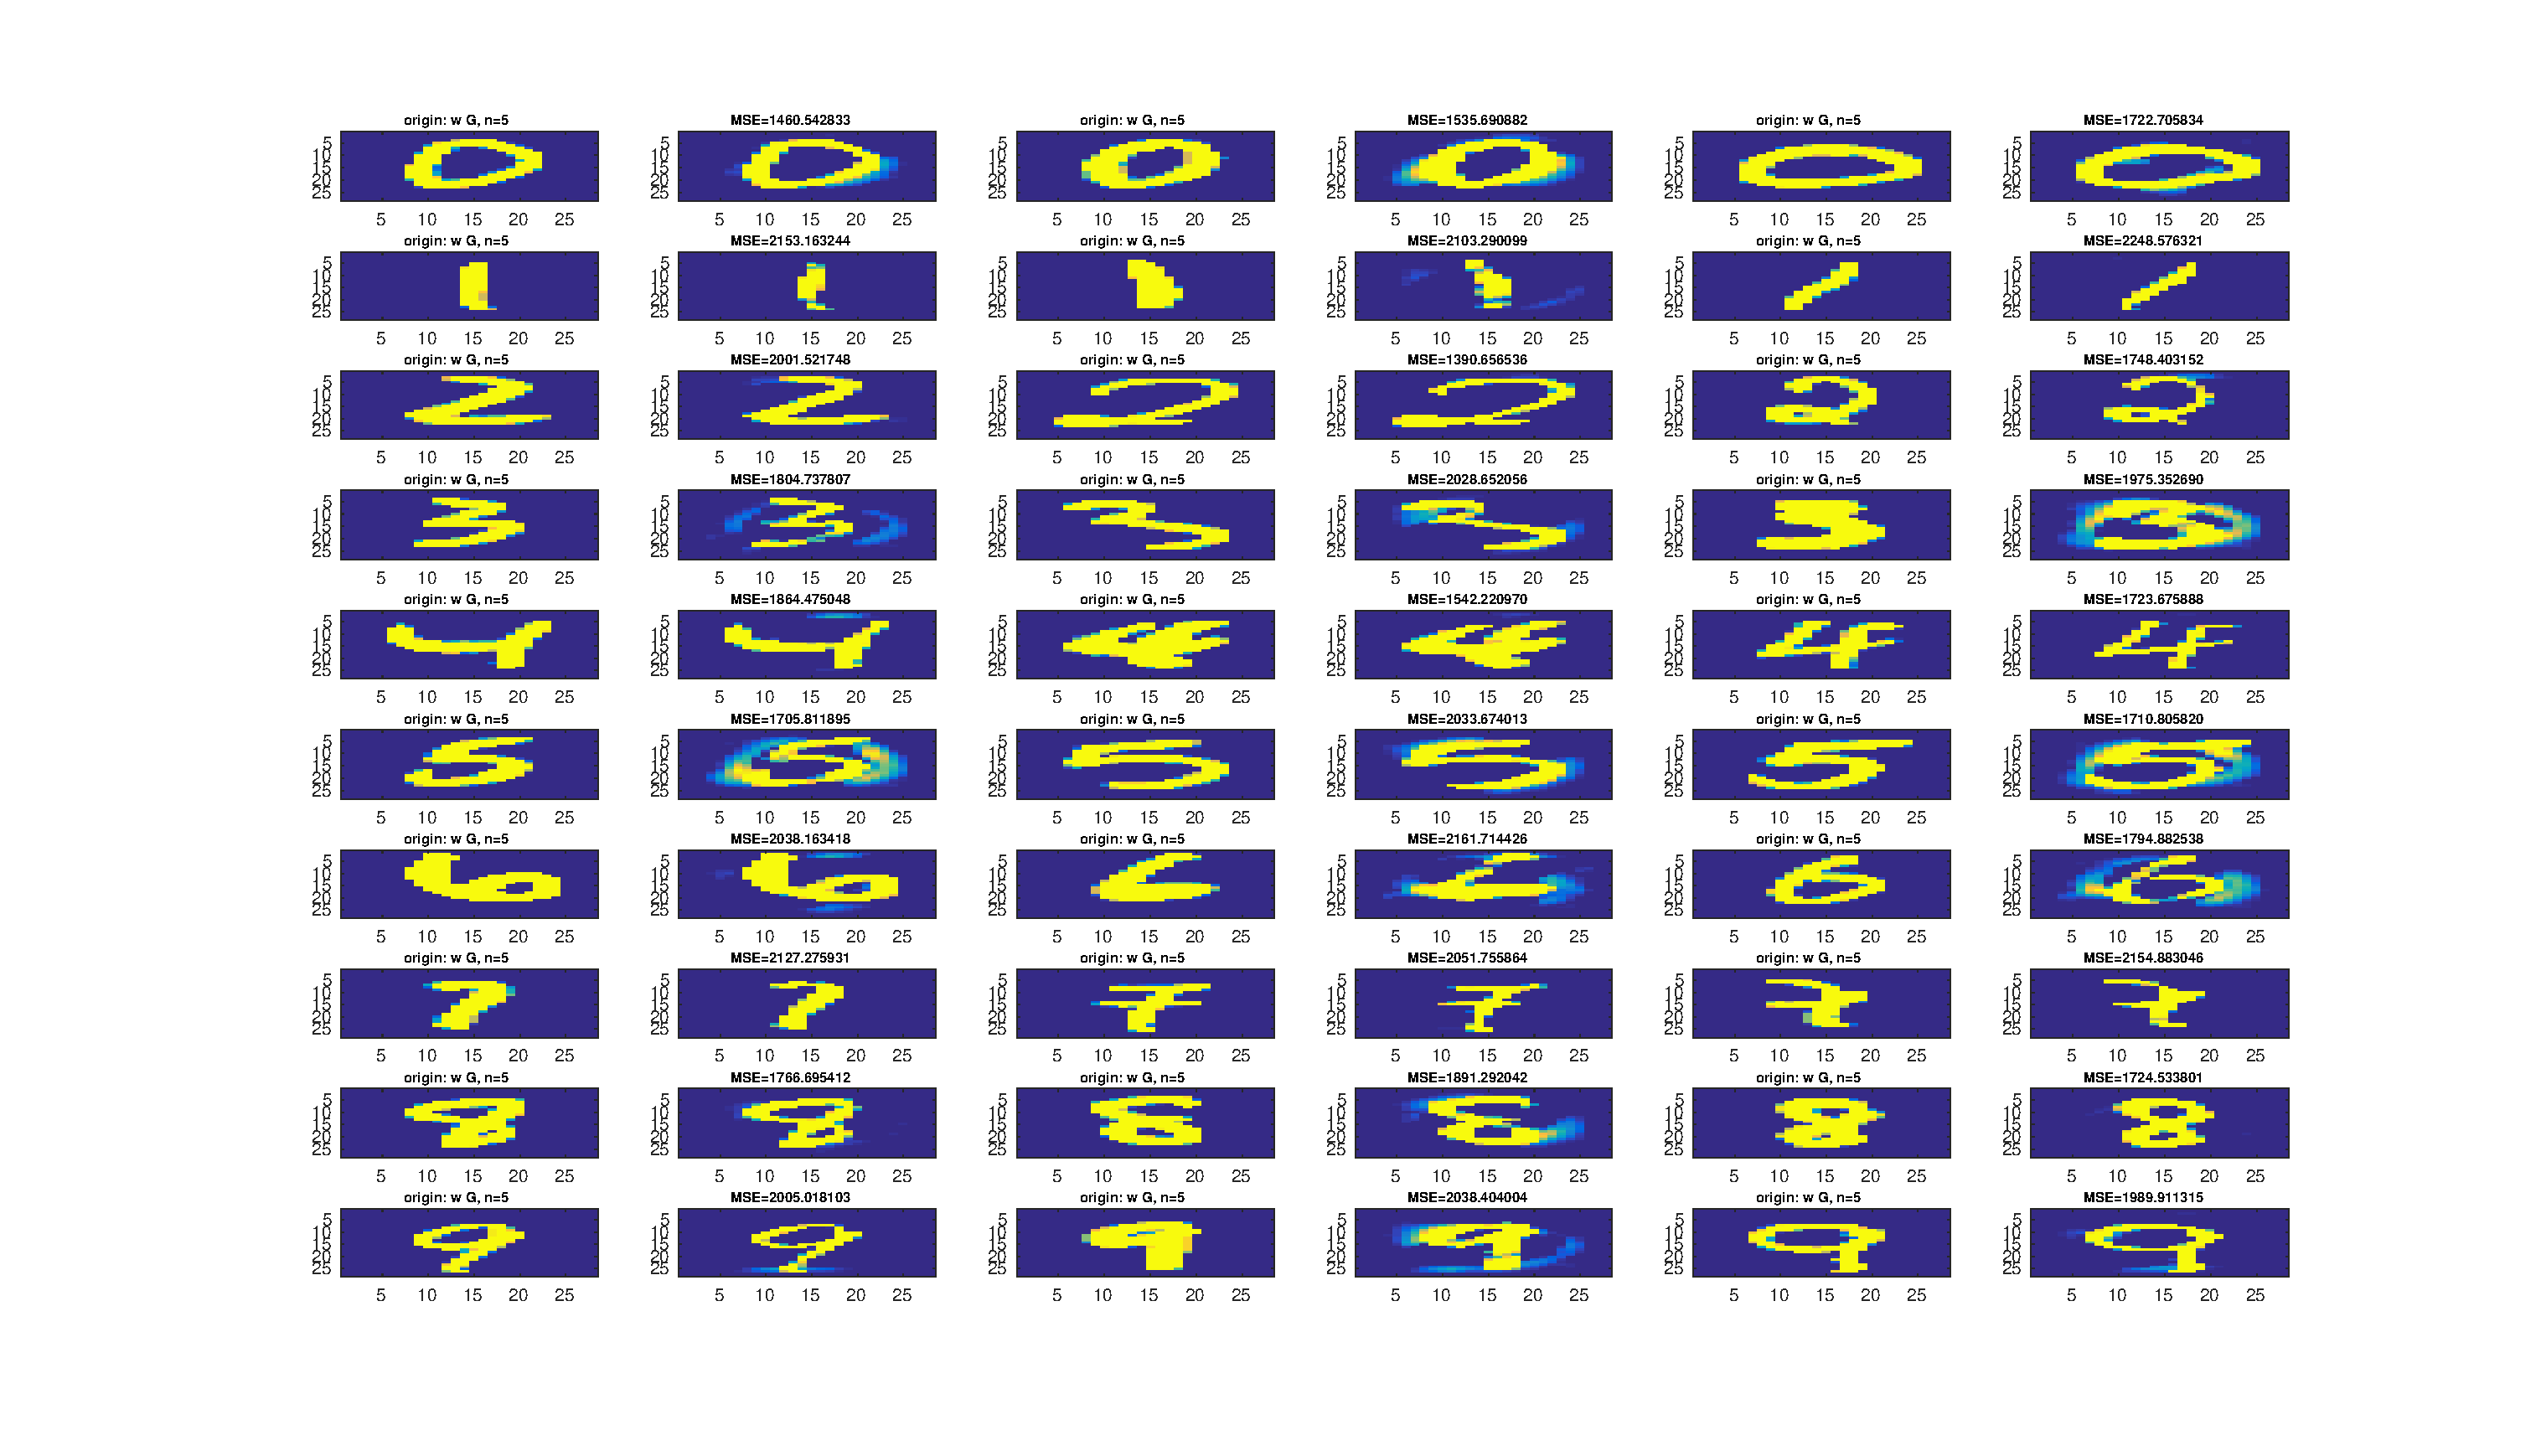
\includegraphics[width=0.95\textwidth]{./matlab/WG_N05.eps}
	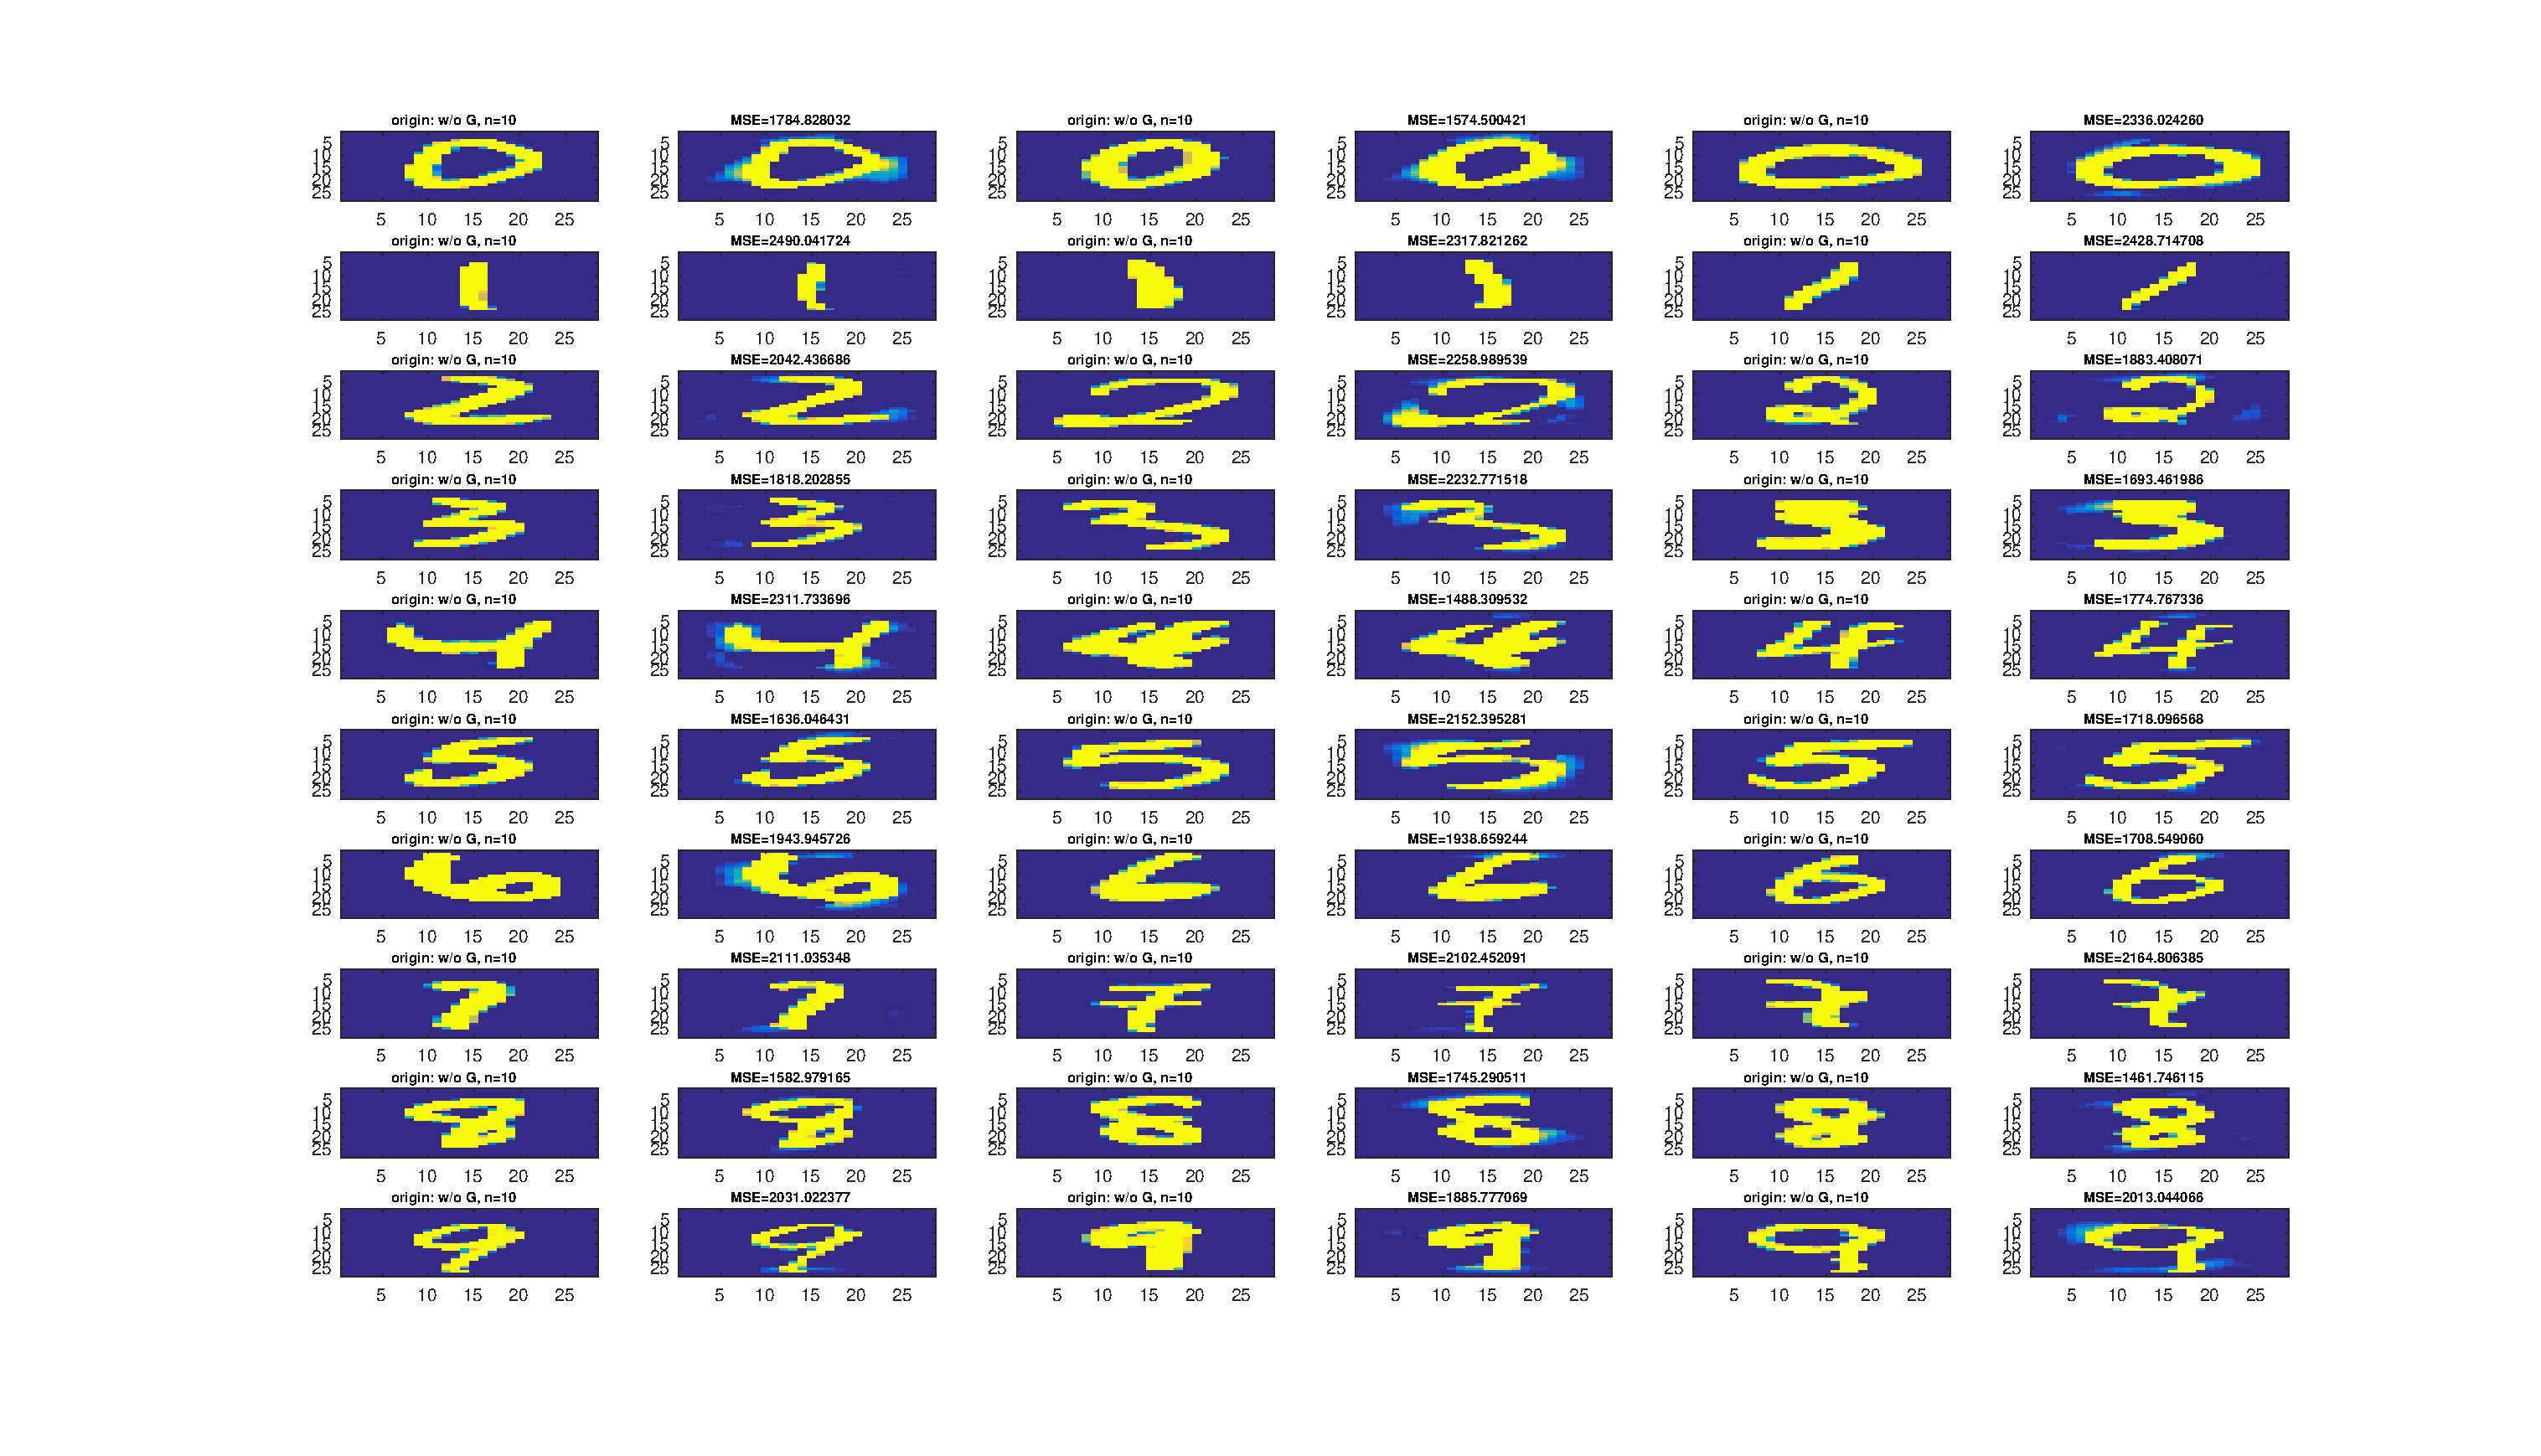
\includegraphics[width=0.95\textwidth]{./matlab/WoG_N10.eps}
	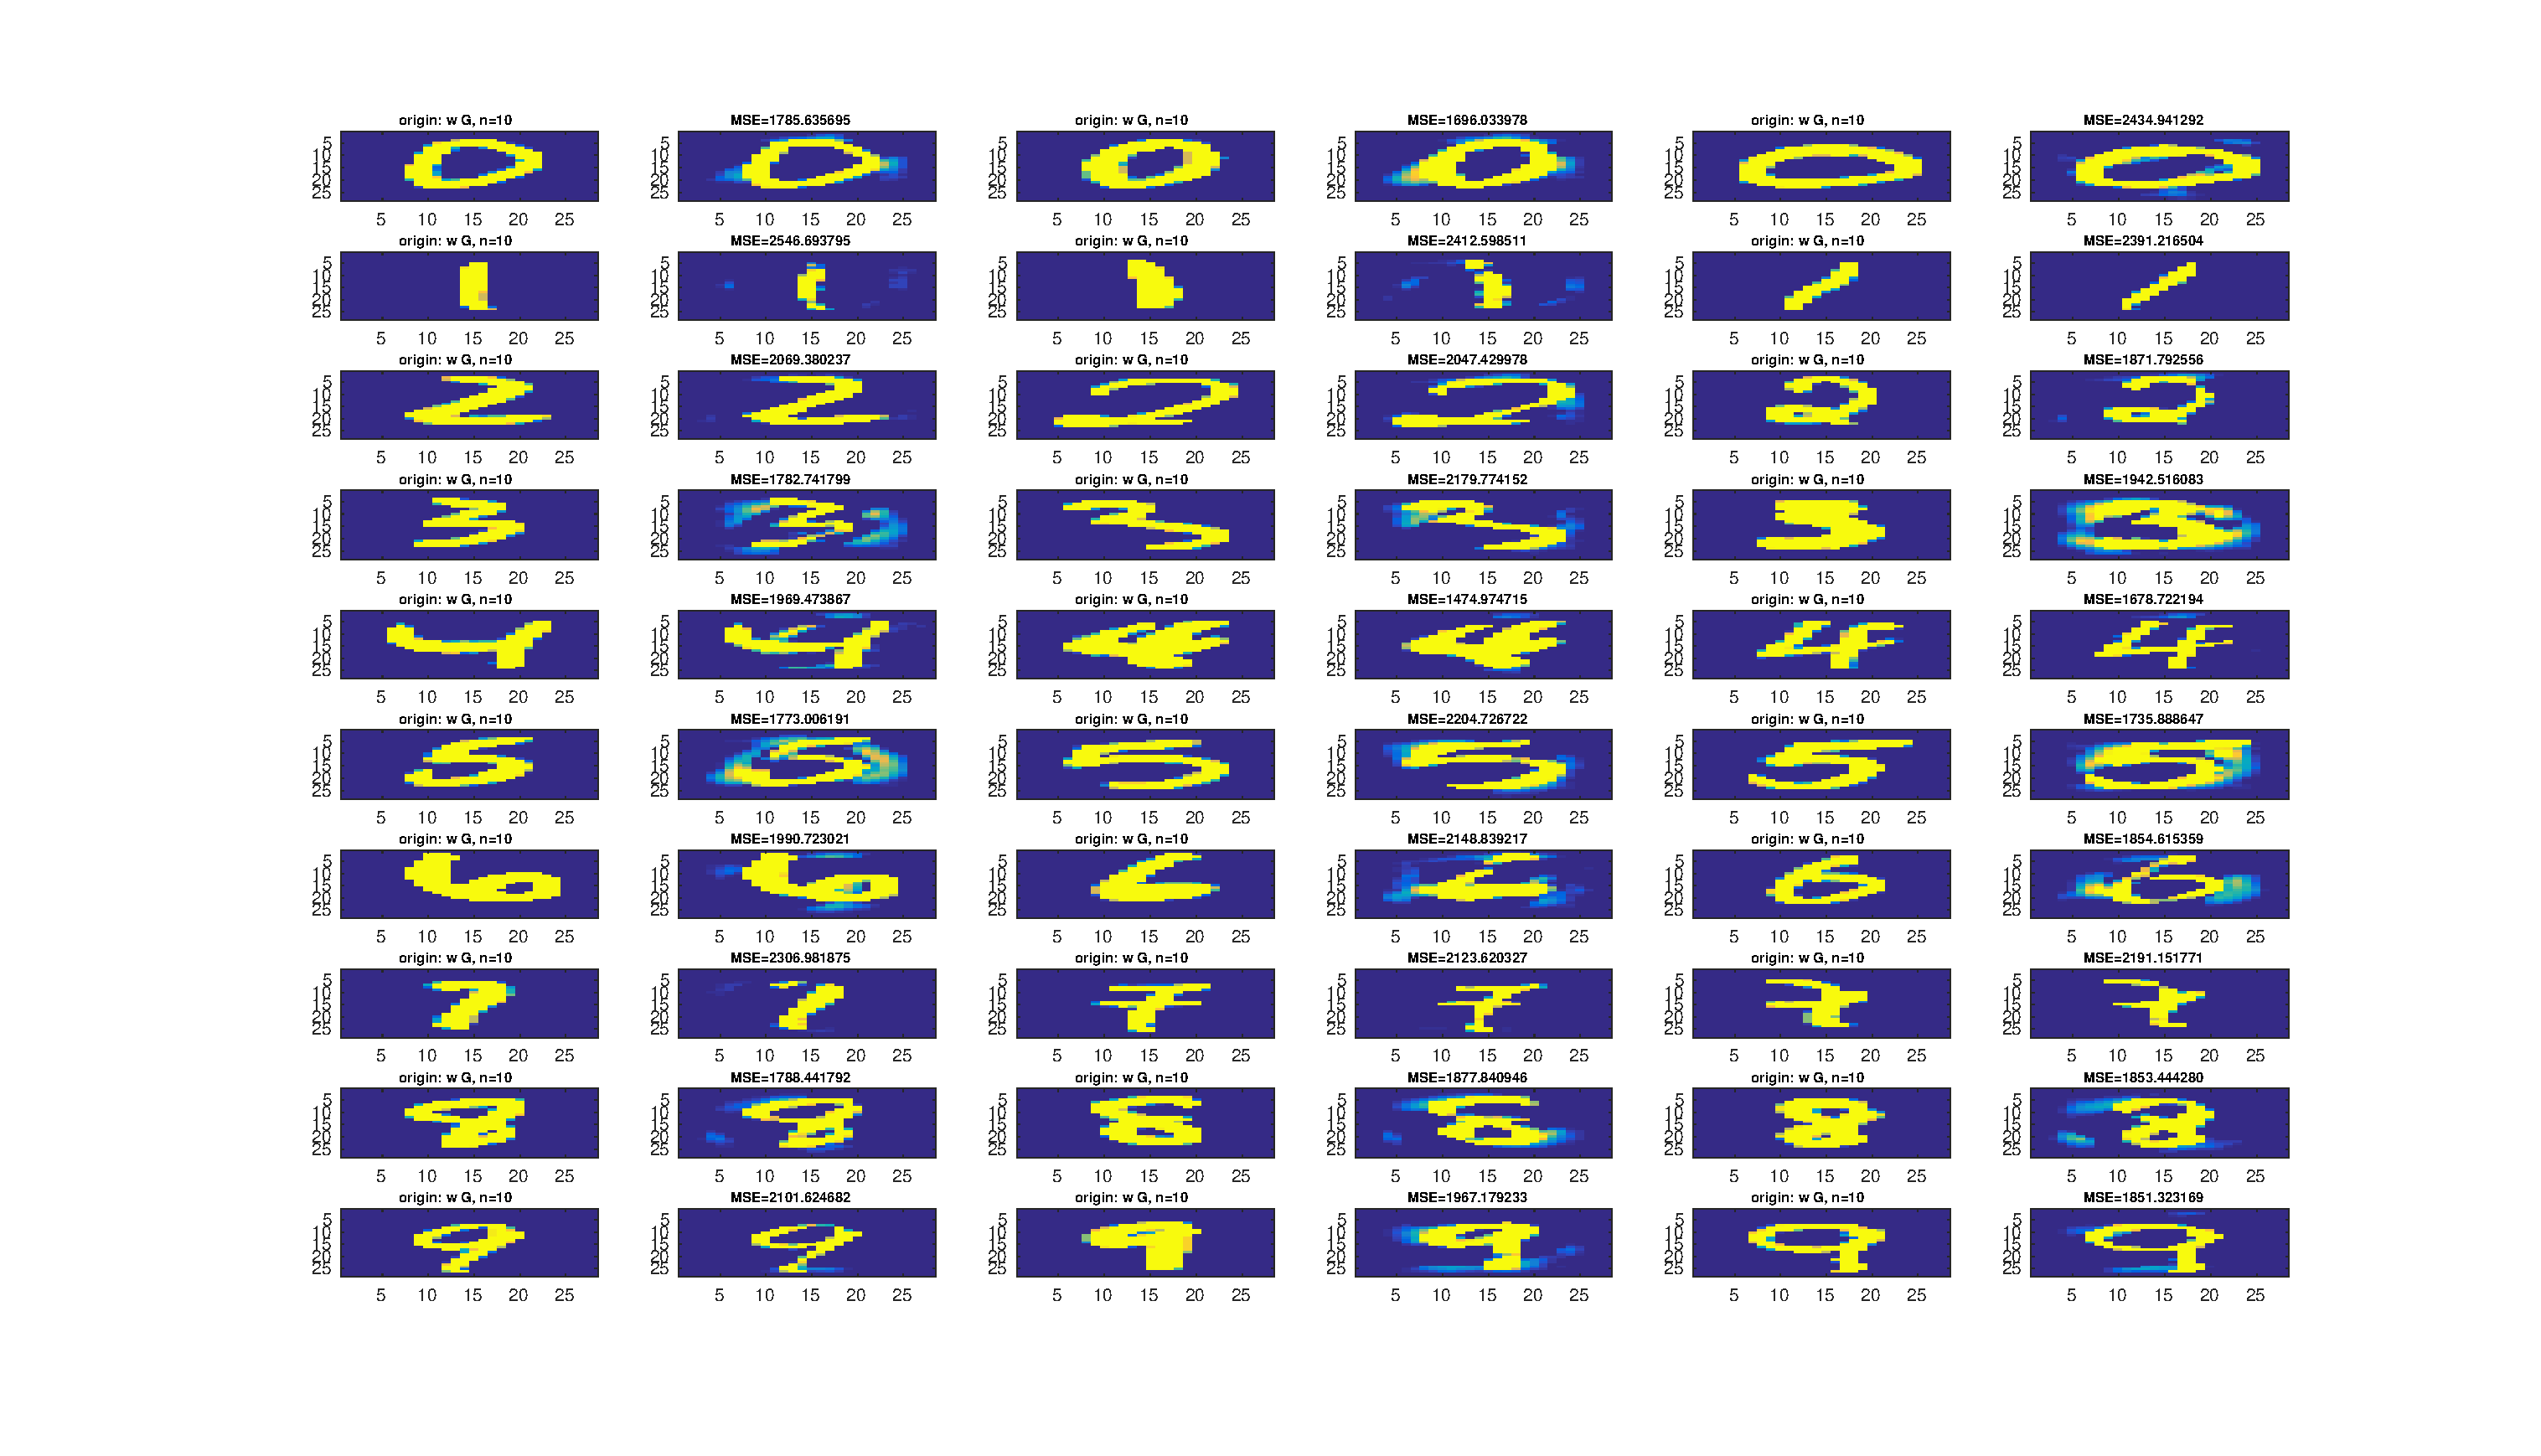
\includegraphics[width=0.95\textwidth]{./matlab/WG_N10.eps}
	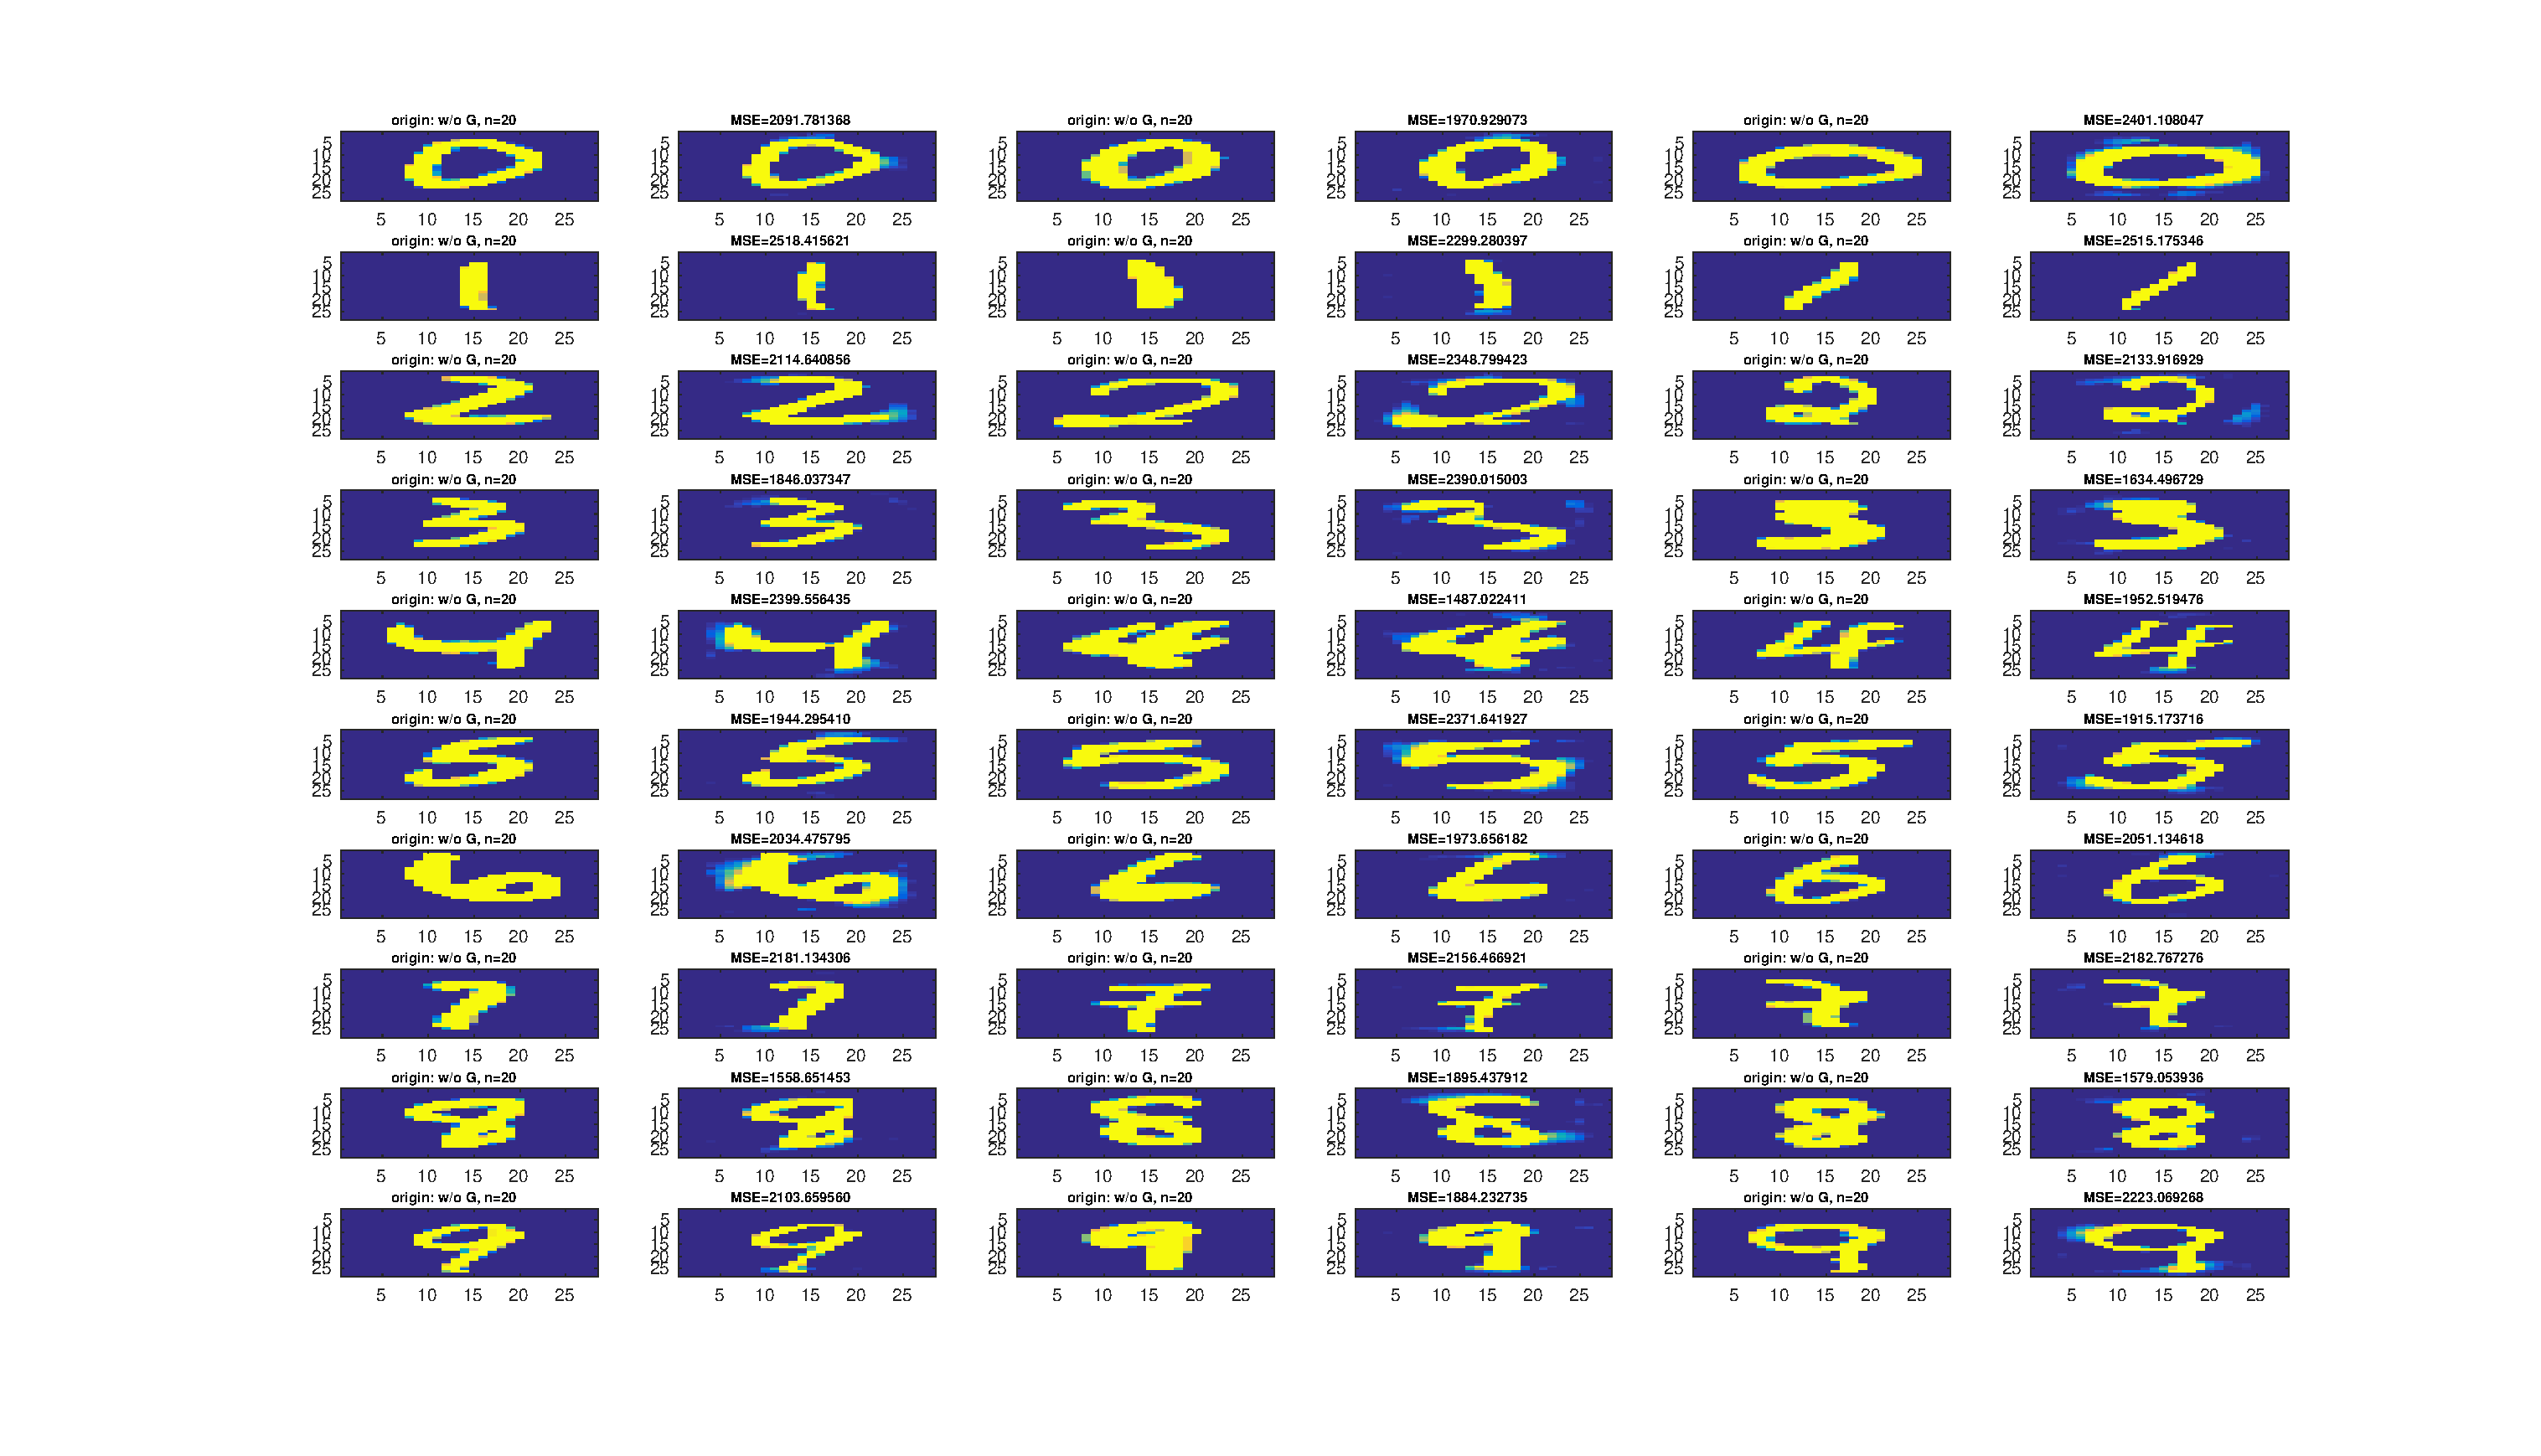
\includegraphics[width=0.95\textwidth]{./matlab/WoG_N20.eps}
	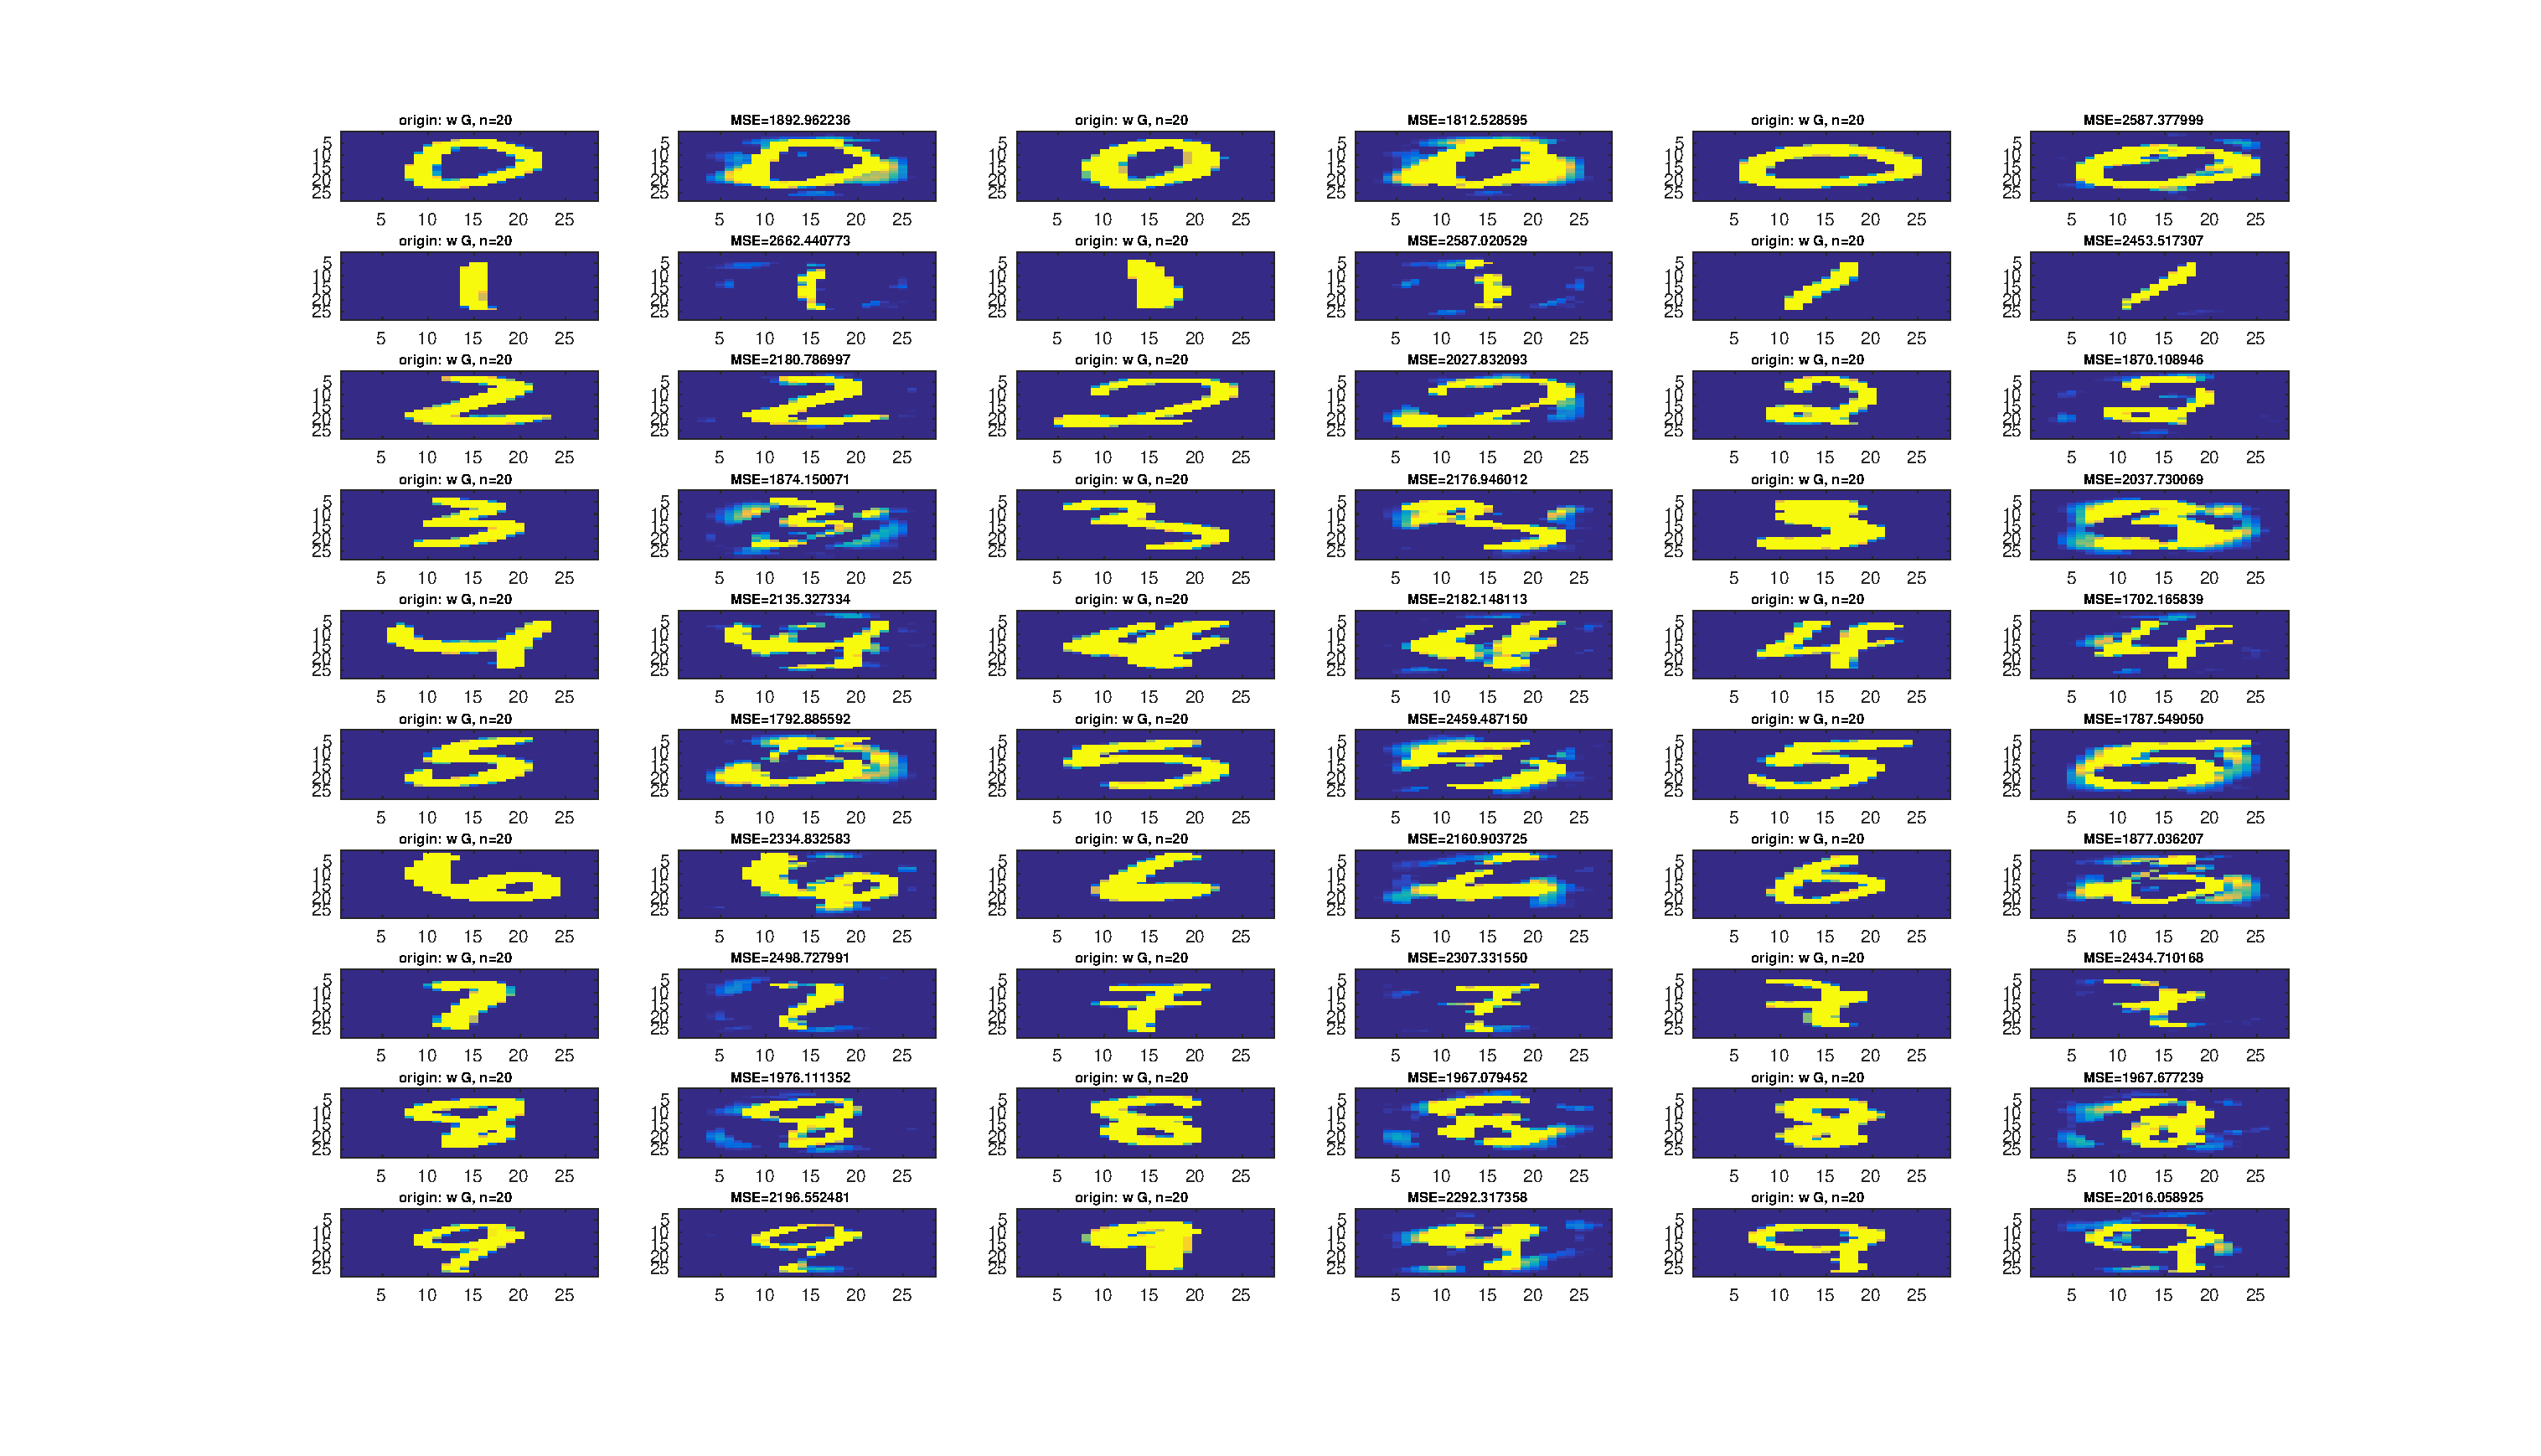
\includegraphics[width=0.95\textwidth]{./matlab/WG_N20.eps}
	\end{center}
	
\end{enumerate}

\end{document}